\documentclass[authoryear,preprint,review,12pt]{elsarticle}

% Pattern Recognition working submission draft.
% The review option supplies the single-column, double-spaced reading layout.
% Replace author, affiliation, funding, and disclosure placeholders before submission.

\usepackage[T1]{fontenc}
\usepackage[utf8]{inputenc}
\usepackage{lmodern}
\usepackage{amsmath,amssymb,booktabs,tabularx,array,longtable}
\usepackage{graphicx,microtype,xcolor}
\usepackage[colorlinks=true,hypertexnames=false,linkcolor=blue!45!black,
  citecolor=blue!45!black,urlcolor=blue!45!black,breaklinks=true]{hyperref}

\journal{Pattern Recognition}
\graphicspath{{./}}
\newcommand{\PrimaryClips}{14,650}
\newcommand{\PrimaryGainMin}{2.37}
\newcommand{\PrimaryGainMax}{8.17}
\newcommand{\EnglishOneNoContext}{47.48}
\newcommand{\EnglishOneContext}{29.98}


\begin{document}

\begin{frontmatter}

\title{Context-Aware Interval Transcription for Visual Speech Recognition}

\author[inst1]{Author information to be inserted}
\ead{corresponding.author@example.org}
\address[inst1]{Affiliation to be inserted, City, Country}

\begin{abstract}
Transcribing a selected video passage requires controlling the returned text while retaining
useful neighboring visual evidence. We formulate context-aware interval transcription by separating
the requested text interval from the permitted observation interval. A training-free implementation,
prediction-aligned projection, recognizes the available context, aligns its predicted tokens using
native visual CTC scores, and returns complete words assigned to the request. We evaluate this
procedure together with crop-first recognition, contextual direct decoding, identical-transcript
allocation controls, and reusable full-clip lookup. Across \PrimaryClips{} clips from four corpora
in three languages, development-selected projection reduces requested-interval error by
\PrimaryGainMin{}--\PrimaryGainMax{} percentage points relative to crop-first recognition.
Matched-decoder comparisons distinguish the benefit of contextual encoding from the additional,
decoder-dependent effect of transcript projection. Real neighboring video also outperforms
equal-length repeated-boundary padding. A 4,006-clip duration study relates these effects to the
context actually available around a request: one-second LRS2 targets improve from
\EnglishOneNoContext{}\% to \EnglishOneContext{}\% WER with up to 0.64 seconds per side.
Repeated-query measurements identify a complementary workload distinction: bounded recognition
can reduce first-query work, while full-clip transcription benefits from reuse and remains stronger
for complete transcripts. The resulting framework connects recognition context, output selection,
and computational reuse for passage-level visual transcription.
\end{abstract}

\begin{highlights}
\item Context admission and requested-output ownership are formulated as separate decisions.
\item Prediction-aligned projection uses a frozen VSR model and native visual CTC scores.
\item Matched decoding separates contextual encoding gains from transcript readout gains.
\item Context availability and query reuse determine the accuracy--workload trade-off.
\end{highlights}

\begin{keyword}
visual speech recognition \sep interval transcription \sep visual context
\sep CTC alignment \sep inference \sep multilingual evaluation
\end{keyword}

\end{frontmatter}

\section{Introduction}

Visual speech recognition (VSR) recovers spoken language from facial motion.
Recent systems learn strong representations from large audiovisual collections and
decode complete utterances with CTC, attention, or combinations of the two
\citep{graves2006ctc,watanabe2017hybrid,ma2023autoavsr}.
Complete-utterance recognition is an important benchmark, but an interface need
not request an entire utterance. A video editor may select a short passage for
transcription, or a viewer may request the speech in a particular time interval.
When audio is unavailable or unsuitable for the task, a visual recognizer must
decide both what context to observe and which recognized words to return.

The obvious solution is to crop the requested interval and run an existing
recognizer. This makes the input boundary coincide with the requested output
boundary. The coincidence is convenient computationally, but may discard useful
speech immediately outside the selection. Neighboring video can help resolve
the target's visual ambiguity or preserve temporal structure near the crop
boundary. However, passing a larger clip to the recognizer introduces another
problem: the resulting transcript includes speech that was not requested.
Context admission and output selection therefore need to be considered together.

We formulate \emph{context-aware interval transcription}: given a requested
interval and an allowance of neighboring video, return the transcript assigned
to the request. The formulation separates two decisions: which frames support
recognition, and where to enforce the output boundary. Contextual direct decoding
restricts contextual encoder states before decoding. Our
\emph{prediction-aligned projection} instead decodes the allowed video, aligns
its predicted tokens with native visual CTC scores, and selects complete words
after recognition. Both procedures use the same contextual input and frozen
recognizer. Their comparison reveals how the stage of output restriction
interacts with decoding.

Three research questions organize the study. First, does genuine neighboring
video improve recognition of a fixed target beyond the effect of input length?
Second, when does selecting from a contextual transcript help beyond selecting
contextual encoder states? Third, how do the context available around a request
and the reuse of earlier computation affect the accuracy--cost tradeoff?
Crop-first recognition, matched decoders, identical-transcript allocation
controls, and full-clip timestamp lookup provide the corresponding comparisons.
The full-clip alternative is particularly relevant when an application can
process the entire video or already holds a transcript index.

The study contributes an interval-transcription formulation and a concrete
prediction-aligned implementation that adapts pretrained VSR to selected-passage
requests. A controlled four-corpus evaluation then separates contextual encoding,
decoder behavior, and temporal output selection. Finally, context interventions,
duration grids, and repeated-query measurements establish an empirical account
of when bounded recognition is useful and when reusable full-clip processing
is preferable. Together, these contributions support passage-level visual
transcription through an explicit treatment of context, output scope, and work
per request.

\section{Related work}

\paragraph{Visual context and recognition units.}
Visual context is already important in lipreading. \citet{stafylakis2018boundaries}
study target-word boundaries and context for word recognition. Sentence recognizers
also learn temporal dependencies over their input, while large-scale automatic
labeling helps expand their training material \citep{ma2023autoavsr,yeo2024vsrlow}.
More recently, GLip learns to combine local and global visual features,
including contextual enhancement, to improve recognition under visual
degradation \citep{wang2025glip}. Such learned feature integration addresses
representation robustness; our study holds the recognizer fixed and varies
the observed interval and returned text scope.
Our question concerns inference with these existing recognizers: how can the
input retain surrounding speech while the returned transcript is restricted to
an arbitrary requested interval? The target is a variable-length unknown text,
rather than a class from a fixed word vocabulary.

\paragraph{Visual alignment and keyword localization.}
\citet{kim2023dvfa} learn to align a supplied transcript with talking-face video
and examine transcript--video mismatches. CTC also supplies a monotonic alignment
structure, and CTC segmentation has been used to associate text with long speech
recordings \citep{graves2006ctc,kurzinger2020segmentation}.
Recognition followed by alignment is also established in speech: WhisperX
combines transcription and forced phoneme alignment to obtain word timestamps
\citep{bain2023whisperx}. We use this general pattern within a frozen visual
recognizer, aligning its own predicted tokens with its native CTC scores.
The contribution lies in evaluating how contextual observation and temporal
output selection interact for interval requests, with separate controls for
context, decoding, and reusable full-clip transcription.

Visual keyword spotting takes a complementary input--output direction.
For example, Transpotter receives a keyword representation and video, then
localizes the keyword if present \citep{prajwal2021transpotter}. Interval
transcription receives a temporal location and predicts its unknown text.
Neither a keyword nor the reference transcript is supplied to our inference
procedure.

\paragraph{Decoder and corpus conditions.}
Hybrid CTC/attention decoding combines monotonic alignment with sequence-level
prediction \citep{watanabe2017hybrid}. Comparisons of VSR decoder families show
that decoder behavior depends on data and training conditions
\citep{gimeno2024decoders}. Spanish VSR experiments further illustrate the
importance of corpus conditions and transfer \citep{gimeno2025spanish}.
Consequently, we report both independently selected systems and matched-decoder
controls. Multilingual corpora such as MuAViC enable evaluation beyond English
\citep{anwar2023muavic}, but differences between languages remain entangled with
corpus composition and checkpoint training. Our cross-corpus results are
replications of an inference comparison, not estimates of a language effect.
Recent evaluations further show sensitivity to evaluation distributions and lexical bias
beyond the standard benchmark \citep{lin2026generalisability}, while isolated-word
experiments identify differences between model and human recognition patterns
\citep{jain2026lipreadinggap}. These findings motivate examining the information
available around a request and the decoder used to interpret it. Our paired
context interventions address that inference question without treating lower
transcription error as evidence of a particular human-like perceptual mechanism.

\paragraph{Efficient and selective inference.}
Efficiency work can reduce the representation or computation used by a speech
model; selective inference instead changes the portion of input needed to answer
a request. We examine this second choice without retraining the backbone.
Its appropriate alternative is a reusable full-clip transcript with timestamps.
The measured workload therefore includes both a first interval request and
multiple requests, rather than assuming that a bounded input is always faster.

\section{Context-aware interval transcription}
\label{sec:method}

\begin{figure}[tb]
 \centering
 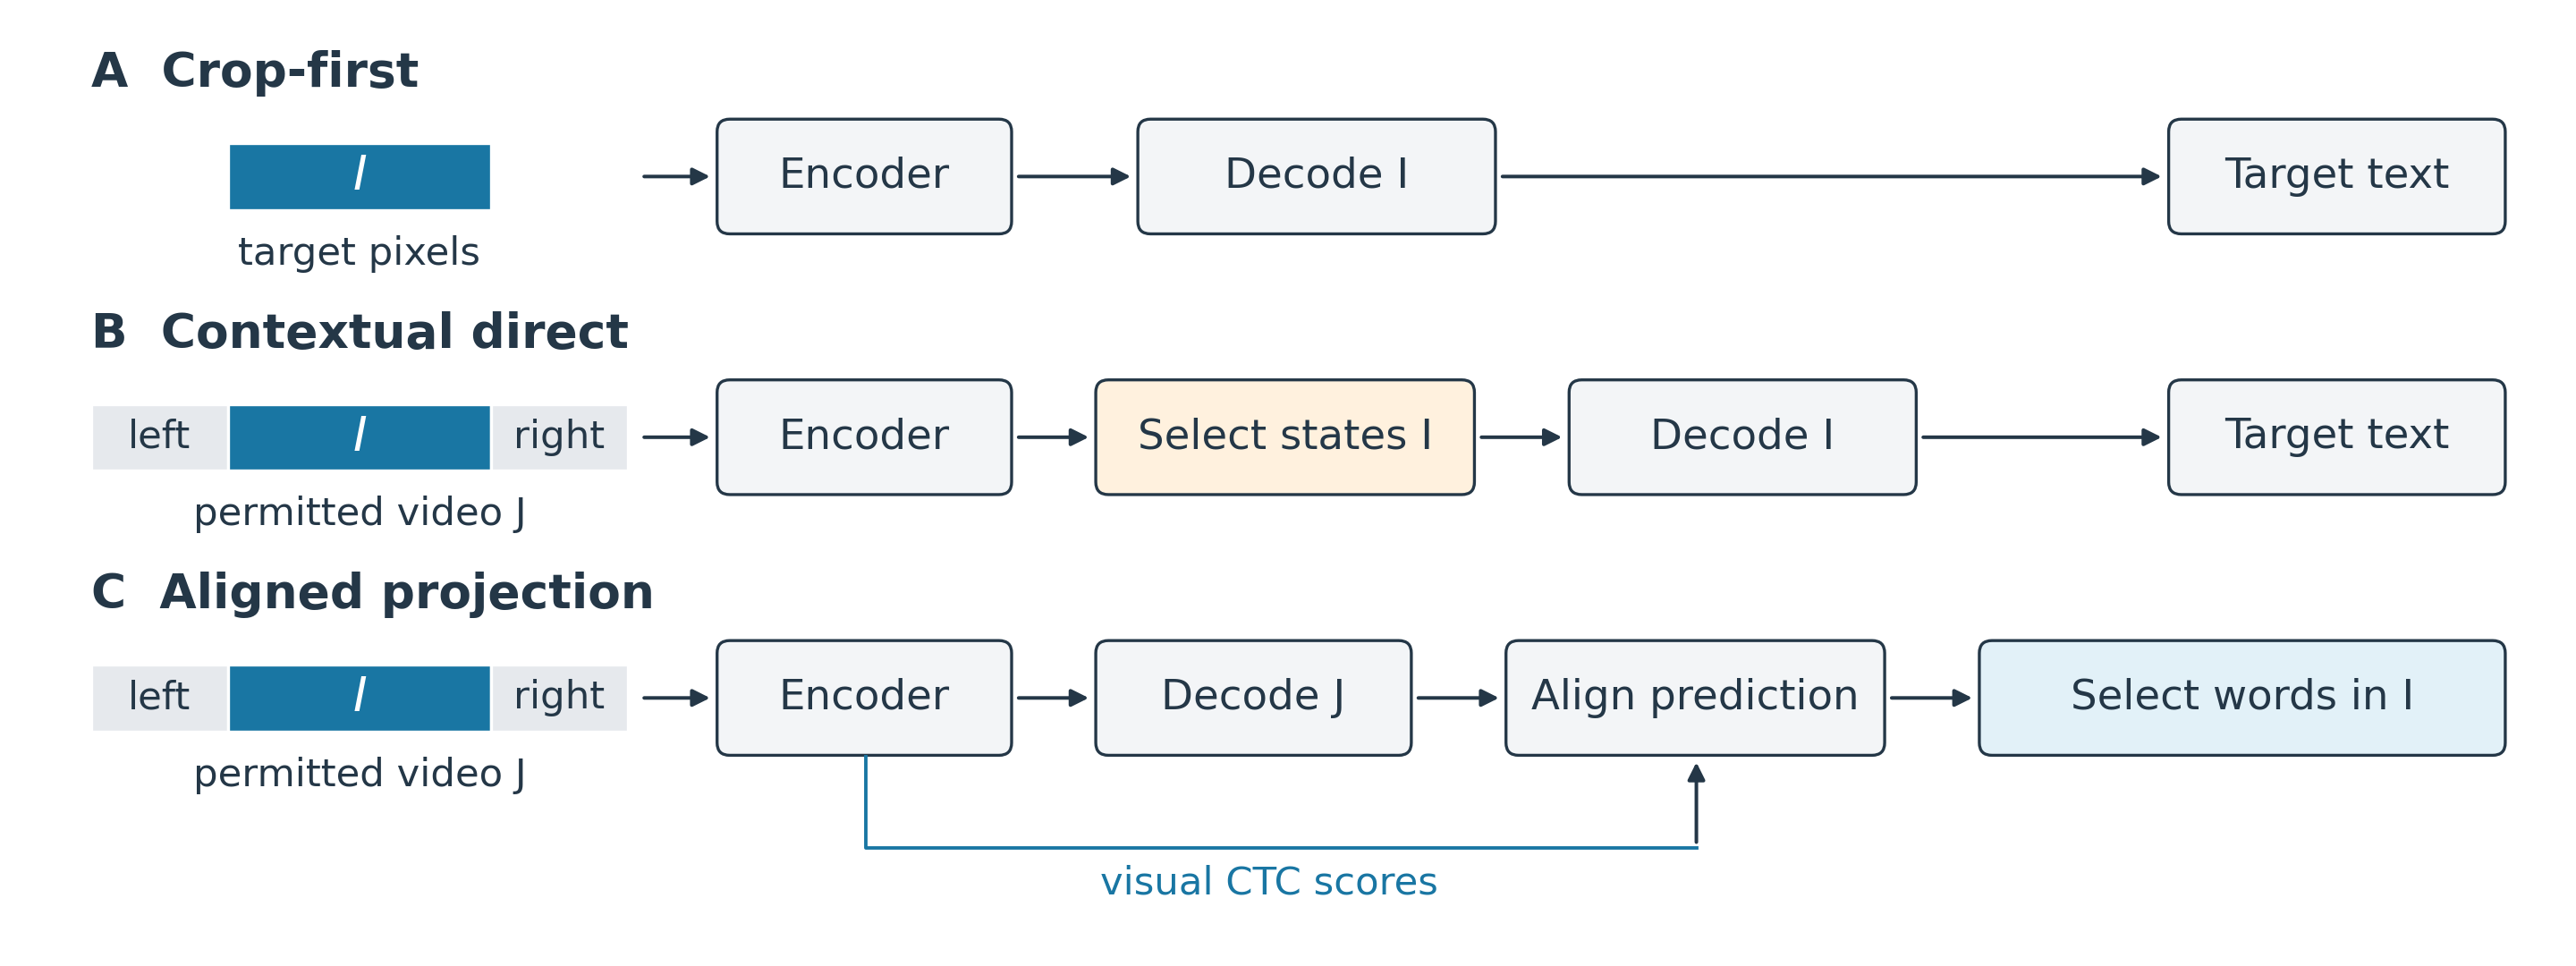
\includegraphics[width=\linewidth]{fig_Interval_Method.png}
 \caption{Three ways to transcribe the same requested interval $I$.
 Crop-first restricts the video before encoding. Contextual direct encodes
 the permitted context $J$ and selects target states before decoding.
 Aligned projection decodes $J$, aligns its own prediction with visual CTC
 scores, and selects words assigned to $I$. B and C observe the same video;
 all alternatives reuse the same frozen recognizer within a corpus.}
 \label{fig:method}
\end{figure}

\subsection{Requested and observed intervals}
Let \(X=(x_0,\ldots,x_{T-1})\) be a prepared mouth-region video, and let
\(I=[a,b)\) be the requested interval in frame coordinates. A context allowance
\((c_{\ell},c_r)\) defines the permitted input
\begin{equation}
 J=[\max(0,a-c_{\ell}),\min(T,b+c_r)).
\end{equation}
The recognizer may observe \(X_J\), while the returned text should belong to
\(I\). Context is real video from the same clip; no frames are fetched beyond its
boundaries. Thus a nominal context budget is an upper bound, and \(J=I\) is
possible for short clips.

Write \(E\) for the visual encoder and \(D\) for a decoder. The encoder also
provides visual CTC token scores \(P_J\). The same pretrained parameters are
used for all inference alternatives within a corpus/model setting.
The experiment distinguishes three operations (Figure~\ref{fig:method}):
\begin{align}
 \widehat{Y}_A &= D(E(X_I)), \label{eq:a}\\
 \widehat{Y}_B &= D\bigl([E(X_J)]_I\bigr), \label{eq:b}\\
 \widehat{Y}_C &= \Pi_I\bigl(D(E(X_J)),P_J\bigr). \label{eq:c}
\end{align}
Crop-first \(A\) restricts pixels before encoding. Contextual direct \(B\)
encodes \(J\), then restricts the decoder to contextual states associated with
\(I\). Projection \(C\) decodes all of \(J\), then restricts the returned words.
Equations~\eqref{eq:b} and~\eqref{eq:c} use the same permitted visual information.
They differ in where the output restriction is applied. The equations motivate
an empirical comparison of state-level and transcript-level readout.

\subsection{Prediction-aligned projection}
The contextual decoder first produces token sequence \(\widehat{z}_J\).
We then align that sequence monotonically to \(P_J\) using a CTC trellis.
Alignment is conditioned on predicted tokens, never on the evaluation
transcript. The recognizer therefore supplies both the text proposal and the
visual scores used to place it.

Tokenizer-aware grouping converts the aligned tokens into complete words.
For a predicted word \(w_k\), the union of its constituent token spans gives
\([s_k,e_k)\) in the contextual input. Its midpoint is mapped back to the
original clip coordinates. Projection returns
\begin{equation}
 \widehat{Y}_C
 = \operatorname{concat}\{w_k:\ a \leq j_0+(s_k+e_k)/2 < b\},
 \label{eq:projection}
\end{equation}
in predicted order, where \(j_0\) is the start of \(J\). Whole words are returned;
the procedure does not cut a subword string at an arbitrary frame.
If the requested interval covers the full available input, the native decoded
transcript is returned directly. This identity case avoids changing ordinary
recognition when there is no outside context.

Projection selects among words in the contextual prediction and preserves
their lexical content and order. It cannot replace a misrecognized word with
the correct word or recover a word omitted by the contextual decoder.
Its role is temporal selection: retaining words assigned to the target and
excluding words assigned outside it. Recognition and temporal assignment thus
jointly determine the returned text. The procedure adds alignment and
allocation work while retaining the pretrained parameters and native CTC head.

\subsection{Controls and unrestricted lookup}
Two allocation controls reuse exactly the same decoded sequence as \(C\).
Uniform-word allocation places its words evenly across \(J\); uniform-token
allocation distributes the predicted tokens evenly and then reconstructs word
spans. Both apply the same midpoint selection rule. Their contrast with \(C\)
isolates the usefulness of predicted visual alignment from the quality of the
generated transcript.

Full-clip lookup \(F\) recognizes \(X\), constructs predicted word times, and
returns words assigned to \(I\). It answers the same target request but has
unrestricted visual input. We also score its complete transcript, as a separate
endpoint, when examining sliding-window recognition. The two endpoints have
different reference denominators and are never treated as interchangeable.

\subsection{Decoder comparability}
We evaluate greedy CTC, pure CTC prefix beam search, and the recognizer's native
hybrid CTC/attention decoding. The pure CTC beam has width 40 and a token-pruning
limit of 64; no external language model is added. Selected-system results use
the decoder chosen for each arm on development data. Matched greedy and pure
CTC results hold that choice fixed across arms.

For hybrid decoding, the output-length cap is derived from the number of
observed frames: \(|I|\) for \(A\), \(|J|\) for \(B/C\), and \(T\) for \(F\).
In particular, \(B\) and \(C\) share the same input-derived cap, although \(B\)
decodes only target states. Greedy and pure CTC use their complete supplied
state sequences rather than an autoregressive cap. Native tokenizer,
normalization, and checkpoint interfaces are retained for each model.

\subsection{Computation across interval requests}
\label{sec:query-computation}
Consider a session with requests \(I_1,\ldots,I_q\), and let
\(\mathcal{J}\) contain their distinct observed intervals. With a fixed
decoder, write \(r(J)\) for recognition cost and \(a(J)\) for the alignment
needed to select words. Ignoring the much smaller selection operation, fresh
projected and full-clip sessions have the respective cost decompositions
\begin{align}
 \tau_C &\simeq \sum_{J\in\mathcal{J}}\bigl[r(J)+a(J)\bigr],\\
 \tau_F &\simeq r([0,T))+a([0,T)).
\end{align}
Alignment is unnecessary when the request covers the entire decoded input.
Exact repeated computations are cached; overlapping but different intervals
are not merged into a shared full-clip encoding. The observed interval set,
rather than the nominal number of requests alone, therefore determines work.
Short clips can make several requested intervals identical.
Distinct targets can also yield the same observed interval after clipping
context at video boundaries. C can then reuse one contextual prediction,
while B may still decode different target-state sequences. Both alternatives
reuse an identical contextual encoding when it is available.

This decomposition links computation to both the observed intervals and their
reuse. B and C encode the same context, while C decodes a larger state sequence
and may require alignment. We measure response cost together with accuracy,
holding the decoder fixed to attribute differences to the inference procedure.

\section{Experimental protocol}
\label{sec:protocol}

\subsection{Corpora, checkpoints, and evaluation units}
The principal assessment contains 11,306 VLR clips, 1,243 LRS2 clips, 934
Spanish clips, and 1,167 ViCocktail clips. VLR and ViCocktail provide two
Vietnamese corpus/model conditions; LRS2 provides English; the Spanish
evaluation uses the MuAViC/mTEDx material
\citep{vlr2026dataset,afouras2022deep,anwar2023muavic,nguyen2025vicocktail}.
The comparison is paired within each corpus and is not pooled across languages.
Recording-source counts are 61, 354, 12, and 20, respectively.
These identifiers group clips from the same source and are not verified
speaker identities.
The prepared clips also differ in duration: means are 5.78 s for VLR, 1.64 s
for LRS2, 5.91 s for Spanish and 5.83 s for ViCocktail. Appendix~\ref{app:corpus}
reports the distributions, actual context availability and recording-source
weights for these exact assessment cohorts.

\begin{figure}[tb]
 \centering
 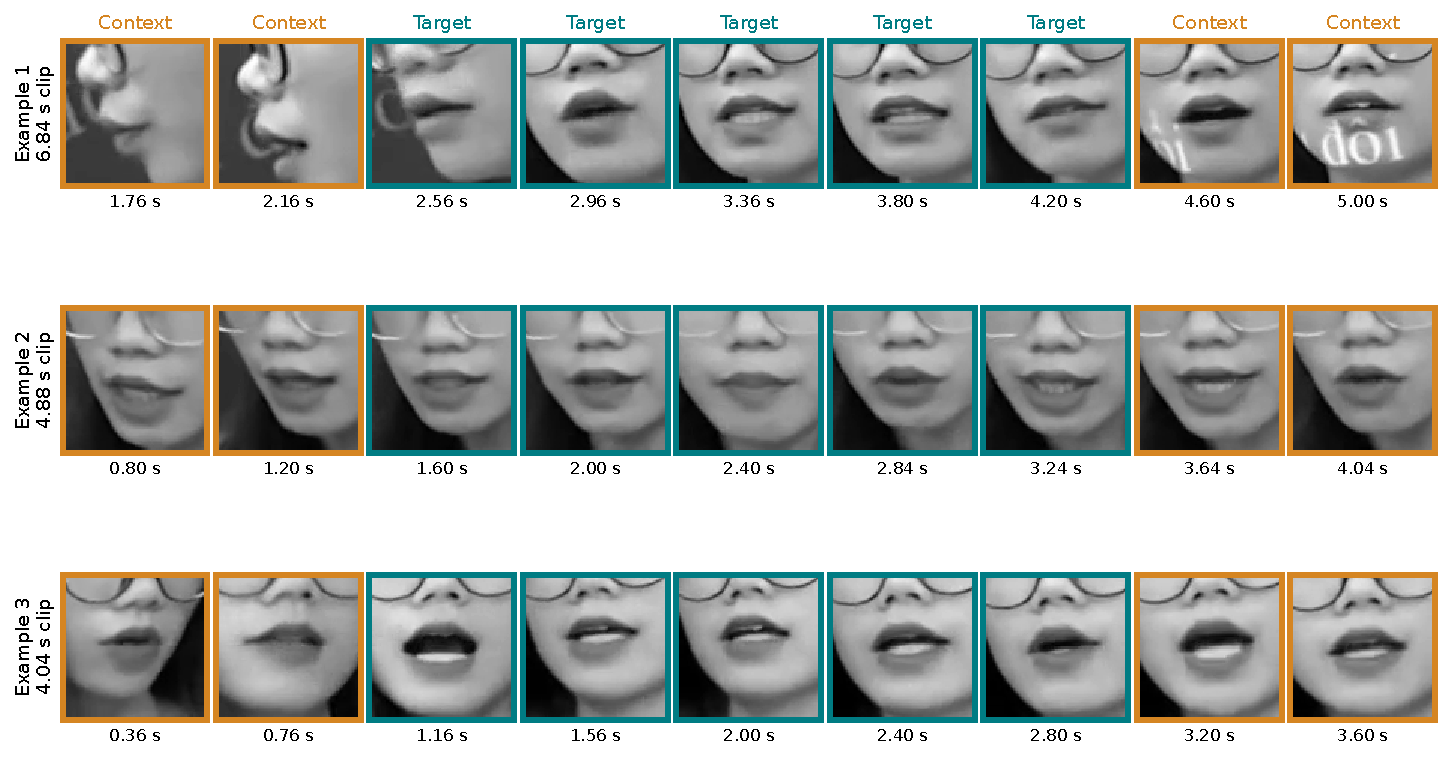
\includegraphics[width=\linewidth]{fig_Dataset_Examples.pdf}
 \caption{Actual prepared VLR mouth-region inputs for three centered requests.
 Each row shows nine sampled frames from an observed interval with a two-second
 target (teal borders) and up to 0.64 seconds of context on each side (orange).
 Times are relative to the original clip. The inputs retain their original
 resolution, motion blur and overlays; they are neither retouched nor generated.
 Examples were selected by clip identifier without using recognition outcomes;
 distinct recording IDs do not imply distinct speakers. Images adapted from
 VLR v2 \citep{vlr2026dataset}, CC BY 4.0.}
 \label{fig:dataset-examples}
\end{figure}

\begin{figure}[tb]
 \centering
 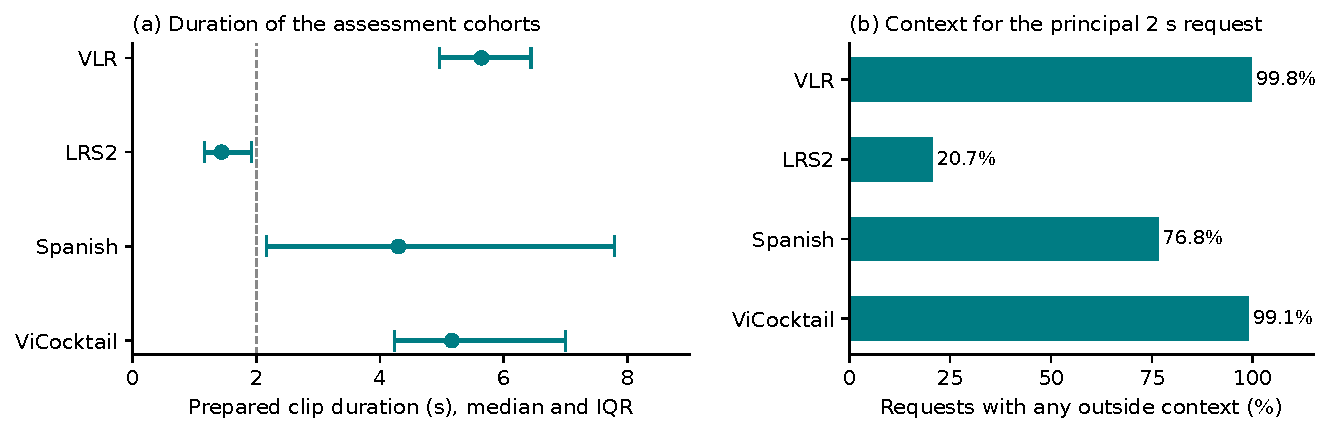
\includegraphics[width=\linewidth]{fig_Corpus_Geometry.pdf}
 \caption{Geometry of the exact four assessment cohorts. (a) Median clip duration
 with interquartile range; the dashed line marks the nominal two-second target.
 (b) Fraction of principal requests with any real video outside their target.
 These are cohort descriptions, not whole-dataset or language-population
 estimates. The short LRS2 clips provide less opportunity to admit context.}
 \label{fig:corpus-geometry}
\end{figure}
Figure~\ref{fig:dataset-examples} illustrates the visual input and the distinction
between target and context. Figure~\ref{fig:corpus-geometry} relates that distinction
to the evaluated clip durations. A context allowance specifies a maximum;
the actual neighboring evidence depends on clip length and request position.

Each setting uses a frozen, language-compatible checkpoint and its native
tokenizer. English uses the published Auto-AVSR visual model trained with
LRS2/LRS3/VoxCeleb2/AVSpeech material \citep{ma2023autoavsr}.
VLR uses our previously adapted T0 checkpoint (seed 17, selected at step 3,000),
and ViCocktail uses our separately trained Vietnamese Auto-AVSR checkpoint
(epoch 13). These are local model instances, not checkpoints released by
the respective dataset authors.
Spanish uses the released \texttt{vsr-low} model of \citet{yeo2024vsrlow},
trained with mTEDx, VoxCeleb2, and AVSpeech material. Its release filename is
\path{es_mted_vox_avs_wer_45.7.pth}; the English release is
\path{vsr_trlrs2lrs3vox2avsp_base.pth}.
The output vocabularies contain 2,002 classes for the two Vietnamese models,
5,049 for English, and 1,006 for Spanish, with the corresponding tokenizer
and special-token conventions retained.
The inference procedure reuses these checkpoints without additional training.

Decoder calibration and assessment are clip- and source-disjoint within the
present protocol. Calibration sizes are 512 for VLR, English, and ViCocktail,
and 286 for Spanish. Assessment membership is frozen before these comparisons.
The material was available during earlier research, so this is an expanded
controlled evaluation rather than a newly collected independent replication.
Eligibility requires usable video and word timing; one VLR clip and 78 of
1,012 Spanish candidate clips are timing-ineligible. No clip is removed because
of its recognition error.

Calibration compares greedy CTC, pure CTC beam search, and hybrid decoding
with CTC weights 0.1, 0.5, and 0.9. Beam searches use width 40 and the
hybrid length bonus is zero. VLR selects greedy decoding for A/B/C and
hybrid weight 0.5 for F. The other three settings select hybrid weight 0.1
for A/C/F and 0.5 for B. Uniform allocation inherits C's prediction and
decoder. These choices are retained throughout the assessment and duration
experiments; matched-decoder comparisons remove this between-arm choice.

We report corpus-level edit error
\begin{equation}
 \mathrm{WER}=100\,\frac{\sum_i(S_i+D_i+I_i)}{\sum_i N_i},
\end{equation}
where the counts refer to the same requested reference text for all compared
arms. Unicode NFC normalization, lowercasing, and whitespace normalization are
fixed. Vietnamese uses whitespace-delimited orthographic units, which need not
coincide with linguistic words. Absolute error rates therefore do not support
a cross-language difficulty ranking.

\subsection{Target construction and reference timing}
The principal setting uses a target of at most 50 frames at 25 fps and up to
16 context frames on either side. Start, center, and end placements are assigned
deterministically from clip identifiers. Clips shorter than the target are
retained as whole-clip targets, rather than excluded to favor context methods.
Within an experimental cell, all arms have the same target reference.

Word midpoints from the fixed reference timing determine target membership.
Whole-clip targets retain the complete original transcript. The reference
transcript and its timing are accessed only for scoring; inference uses video,
predicted tokens, and predicted alignment. VLR retains the supplied
ASR-derived transcript and word spans. LRS2 and Spanish use audio-CTC
forced alignment of their corpus transcripts; ViCocktail uses its native
test labels, reported as manually transcribed by the dataset authors,
with audio-CTC word alignment. Audio is used only to prepare evaluation
references, never by the visual recognizer or prediction-alignment procedure.
These automatic word times are not independent human boundary annotations.
Reference-clock perturbations of \(\pm40,\pm80,\pm160\) ms and an overlap-based
ownership convention examine sensitivity to this evaluation choice.

\subsection{Controlled experiments}
The duration experiment varies nominal target length over 1, 2, and 3 seconds
and maximum context per side over 0, 0.32, and 0.64 seconds. It includes 1,024
clips each for VLR, LRS2, and ViCocktail, and all 934 eligible Spanish clips.
The decoder choices remain those calibrated at the principal operating point;
each duration cell is evaluated without selecting a new decoder.
Within each target
length, it compares the same clips and requested text. Changing target length
changes the reference content, so the smallest raw WER across lengths is not
interpreted as an optimal segmentation duration.

Context interventions use 256 clips per corpus. They compare real context
with equal-length repeated-boundary padding, reversed margins, and left-only
or right-only context while preserving target pixels. The primary padding
contrast uses clips that actually have outside context.
The full-transcript experiment uses 512 clips per corpus. For nominal target
budget \(L\), a clip of \(T\) frames is partitioned into
\(K=\lceil T/L\rceil\) balanced, nonoverlapping target intervals. Direct and
projected sliding share that schedule and concatenate their outputs in time
order. A further control joins contextual target CTC scores before decoding
once, separating text concatenation from repeated local recognition.

For query costs, 32 duration-stratified calibration clips per corpus are
evaluated on a GTX 1650 Ti in float32, at batch size one with two CPU threads
and one GPU worker. One, three, and five
requested intervals are deduplicated when short clips yield identical queries.
Development-selected systems and a separate matched pure-CTC control use
the exact same clips and query schedules. In the matched control, every arm
uses beam width 40 and token-pruning limit 64 without decoder recalibration.
Three fresh sessions are run per scenario, with arm order rotated by clip
and repetition. We first take within-clip medians, then summarize their
median and 95th percentile across clips. Recognition and required allocation are timed
with the model resident; input loading is measured separately. The experiment
also measures repeat lookup from populated caches. It does not measure
raw-video face tracking, live acquisition delay, or human editing time.

\subsection{Uncertainty and comparison families}
The eight principal contrasts are projection versus crop-first and projection
versus contextual direct in each corpus. We use paired source-cluster
bootstrap resampling with 10,000 draws. Bonferroni adjustment gives
99.375\% individual percentile intervals for this family. The interval
construction was chosen at analysis time for the fixed comparison family;
it has approximate bootstrap coverage. Other intervals describe explanatory
contrasts at pointwise 95\% coverage. Limited source counts, especially in
Spanish, constrain the precision and generality of those comparisons.

An explanatory analysis recomputes matched greedy and pure-CTC intervals
from the frozen predictions and partitions each cohort by actual outside
context: none, left only, right only, or both. These post-hoc explanatory
comparisons use the same 10,000-draw paired-source procedure with pointwise
95\% intervals; they do not alter the primary comparison family or decoder
selection. Geometry is read from the recorded input and target coordinates.

\section{Results}

\subsection{Context improves requested-interval recognition}
\begin{table}[tb]
\centering\small
\caption{Requested-interval WER (\%). Each arm uses its development-selected decoder. Targets are at most two seconds with up to 0.64 s of context per side. Source clusters are recording identifiers, not verified speakers.}
\label{tab:primary}
\begin{tabular}{lrrrrr}
\toprule
Corpus & Clips & Sources & Crop A & Direct B & Projection C \\
\midrule
VLR & 11,306 & 61 & 58.602 & 50.579 & 50.434 \\
LRS2 & 1,243 & 354 & 24.099 & 23.609 & 21.733 \\
Spanish & 934 & 12 & 85.451 & 81.527 & 80.170 \\
ViCocktail & 1,167 & 20 & 51.767 & 49.179 & 48.193 \\
\bottomrule
\end{tabular}
\end{table}

\begin{table}[tb]
\centering\small
\setlength{\tabcolsep}{4pt}
\caption{Matched-decoder requested-interval WER (\%). Negative C--B favors projection. Brackets give explanatory pointwise 95\% paired-source bootstrap intervals from 10,000 draws; the primary adjusted family is reported separately.}
\label{tab:matched}
\begin{tabular}{llrrrl}
\toprule
Corpus & Decoder & A & B & C & C--B [95\% CI] (pp) \\
\midrule
VLR & Greedy & 58.602 & 50.579 & 50.434 & -0.145 [-0.181, -0.110] \\
VLR & Pure CTC & 58.971 & 50.862 & 50.691 & -0.172 [-0.214, -0.129] \\
LRS2 & Greedy & 30.527 & 28.749 & 28.471 & -0.277 [-0.463, -0.126] \\
LRS2 & Pure CTC & 30.250 & 28.536 & 28.226 & -0.310 [-0.500, -0.155] \\
Spanish & Greedy & 83.181 & 81.824 & 80.870 & -0.954 [-1.390, -0.672] \\
Spanish & Pure CTC & 83.203 & 81.718 & 80.764 & -0.954 [-1.429, -0.670] \\
ViCocktail & Greedy & 55.540 & 52.643 & 52.524 & -0.119 [-0.213, -0.011] \\
ViCocktail & Pure CTC & 55.520 & 52.623 & 52.464 & -0.159 [-0.249, -0.061] \\
\bottomrule
\end{tabular}
\end{table}

Projection improves over crop-first recognition in all four principal
comparisons (Table~\ref{tab:primary}). The reduction ranges from
\PrimaryGainMin{} to \PrimaryGainMax{} percentage points, and all four
family-adjusted intervals favor projection. The result concerns the same
requested target within each corpus: it is not a comparison between a short
target transcript and a longer full-clip transcript.

Contextual direct decoding captures much of the benefit. For VLR, moving from
crop-first to contextual direct changes WER from 58.602\% to 50.579\%;
projection provides a further 0.145-point reduction. The additional
selected-system reductions are 1.876 points on LRS2, 1.357 on Spanish, and
0.986 on ViCocktail. The adjusted Spanish C--B interval includes zero;
the other three adjusted intervals favor C.

Matched decoders give a more specific interpretation
(Table~\ref{tab:matched}). Under pure CTC, the C--B improvements are
0.172, 0.310, 0.954, and 0.159 points, with explanatory paired-source 95\%
intervals favoring C in all four settings. Thus projection contributes beyond
contextual state cropping at the principal operating point, while contextual
encoding accounts for the larger improvement. The selected-system comparisons
add the effect of each arm's development-selected decoder. Spanish illustrates
the relevance of both views: crop-first greedy and pure CTC outperform its
selected hybrid on assessment.

\paragraph{Decoder sensitivity.}
Projection does not outperform contextual direct at every decoder setting.
On the separate VLR development screen, pure CTC with zero blank bias gives
60.085\% for C versus 59.659\% for B: a C--B difference of +0.426 points
with pointwise 95\% interval [+0.105, +0.802]. VLR greedy decoding also
favors B by point estimate at all three tested blank biases.
On ViCocktail, a hybrid length bonus of +1 gives 45.302\% for C versus
44.214\% for B (+1.088 points, interval [-0.340, +2.739]); this comparison
retains the respective CTC weights of 0.1 and 0.5. These development results
show that the readout ranking depends on decoder configuration. They do not
retune or replace the frozen assessment results (Appendix~\ref{app:decoder-sensitivity}).

\subsection{Actual context availability explains aggregate readout effects}
\label{sec:availability}
\begin{figure}[tb]
 \centering
 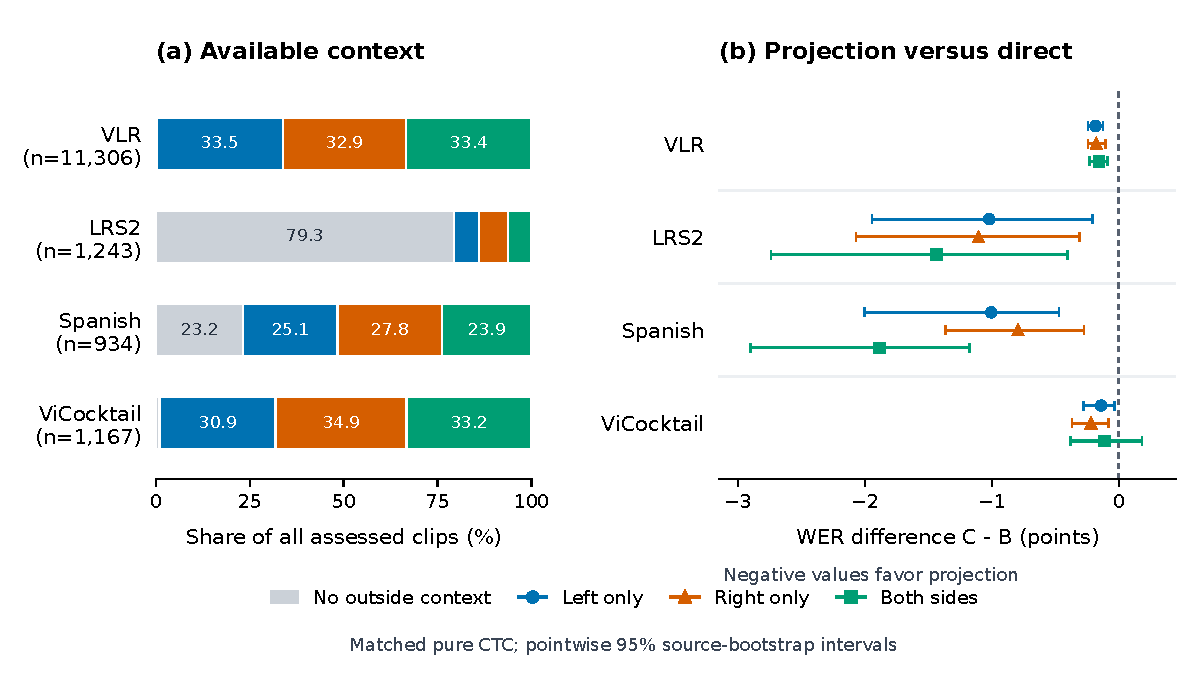
\includegraphics[width=\linewidth]{fig_Context_Availability.pdf}
 \caption{Post-hoc analysis of the frozen principal assessment, using the
 same pure-CTC decoder for A/B/C. (a) All clips partitioned by actual context
 outside the target. (b) C--B WER differences within the three groups with
 outside context; negative values favor projection. Bars are pointwise 95\%
 paired-source bootstrap intervals, without multiplicity adjustment. No-context
 predictions are identical across A/B/C. Groups differ in request position and
 clip duration, so their differences do not isolate causal left/right effects.
 Full counts and WERs appear in Table~\ref{tab:context-availability}.}
 \label{fig:context-availability}
\end{figure}
A post-hoc stratification separates requests by actual outside context
(Figure~\ref{fig:context-availability}; Table~\ref{tab:context-availability}).
With matched decoders, A/B/C predictions are identical when the request covers
the available video. This occurs on
986 of 1,243 LRS2 clips (79.3\%), compared with 27/11,306 VLR, 217/934 Spanish,
and 11/1,167 ViCocktail clips. The LRS2 aggregate thus mixes many identity
cases with requests that permit contextual readout.

For the LRS2 groups with left, right, and both-sided context (83, 96, and
78 clips), the pure-CTC C--B reductions are 1.020, 1.106, and 1.434 points;
each corresponding pointwise interval favors C. The reductions across these
three groups range from 0.158 to 0.183 points on VLR and from 0.794 to
1.883 on Spanish. ViCocktail has smaller reductions of 0.115--0.220 points,
and its both-context interval includes zero. The complete principal endpoint
retains all clips, including those without outside context. This explanatory
analysis uses pointwise 95\% intervals on previously evaluated data; it is
not an independent confirmation or a change to the primary comparison family.
Directional effects of context are tested separately by the interventions below.

\subsection{Visual alignment contributes to output selection}
\begin{table}[tb]
\centering\small
\caption{Development-selected requested-interval WER (\%). The uniform controls allocate the same decoded sequence as C. Full-clip lookup processes unrestricted input and returns the same requested target; it is a different input-budget baseline.}
\label{tab:allocation}
\begin{tabular}{lrrrr}
\toprule
Corpus & Aligned C & Uniform words & Uniform tokens & Full-clip lookup \\
\midrule
VLR & 50.434 & 56.168 & 56.066 & 42.720 \\
LRS2 & 21.733 & 22.842 & 23.071 & 21.553 \\
Spanish & 80.170 & 82.821 & 82.694 & 78.770 \\
ViCocktail & 48.193 & 52.125 & 52.364 & 45.495 \\
\bottomrule
\end{tabular}
\end{table}

Table~\ref{tab:allocation} compares allocation rules applied to the same
contextual prediction. Aligned projection has lower error than both uniform
rules in each principal setting. This comparison cannot be explained by a
different generated transcript: the alternatives share predicted tokens and
differ only in their assignment to the requested interval.

Unrestricted full-clip lookup has the lowest target error in these settings.
It provides the accuracy reference when the application can process the entire
video. The bounded alternatives answer the same request using a prescribed
observation interval, exposing the accuracy cost of that input constraint.

\subsection{Real context supplies more than additional frames}
\begin{table}[tb]
\centering\small
\caption{Real context versus repeated-boundary padding, restricted to clips with available outside context. Both conditions preserve target pixels and input length. Intervals are explanatory pointwise 95\% source-bootstrap intervals.}
\label{tab:intervention}
\begin{tabular}{llrl}
\toprule
Corpus & Decoder regime & Clips & Real--repeat difference (pp) \\
\midrule
VLR & Selected & 254 & -4.219 [-5.905, -2.605] \\
VLR & Pure CTC & 254 & -4.430 [-6.026, -2.913] \\
LRS2 & Selected & 48 & -7.767 [-14.286, -2.222] \\
LRS2 & Pure CTC & 48 & -7.443 [-12.333, -2.857] \\
Spanish & Selected & 202 & -9.635 [-11.979, -7.156] \\
Spanish & Pure CTC & 202 & -3.043 [-4.700, -1.230] \\
ViCocktail & Selected & 254 & -9.286 [-11.456, -7.326] \\
ViCocktail & Pure CTC & 254 & -6.066 [-8.193, -4.103] \\
\bottomrule
\end{tabular}
\end{table}

On clips with outside context, real video improves over repeated-boundary
padding under both selected systems and matched pure CTC
(Table~\ref{tab:intervention}). The target pixels and input length are
unchanged in this contrast. Thus the benefit is not explained solely by a
longer tensor or a different target crop.
The complete intervention table in Appendix~\ref{app:context-controls}
also compares single-sided and reversed context. Both real margins outperform
either margin alone in those settings, while the preferred individual side
varies across corpus/model conditions.

These interventions establish the value of real neighboring content over the
tested alternatives. They affect motion continuity together with speech
information, so the contrast concerns visual context as a whole.

\subsection{Duration changes the opportunity to use context}
\begin{figure}[tb]
 \centering
 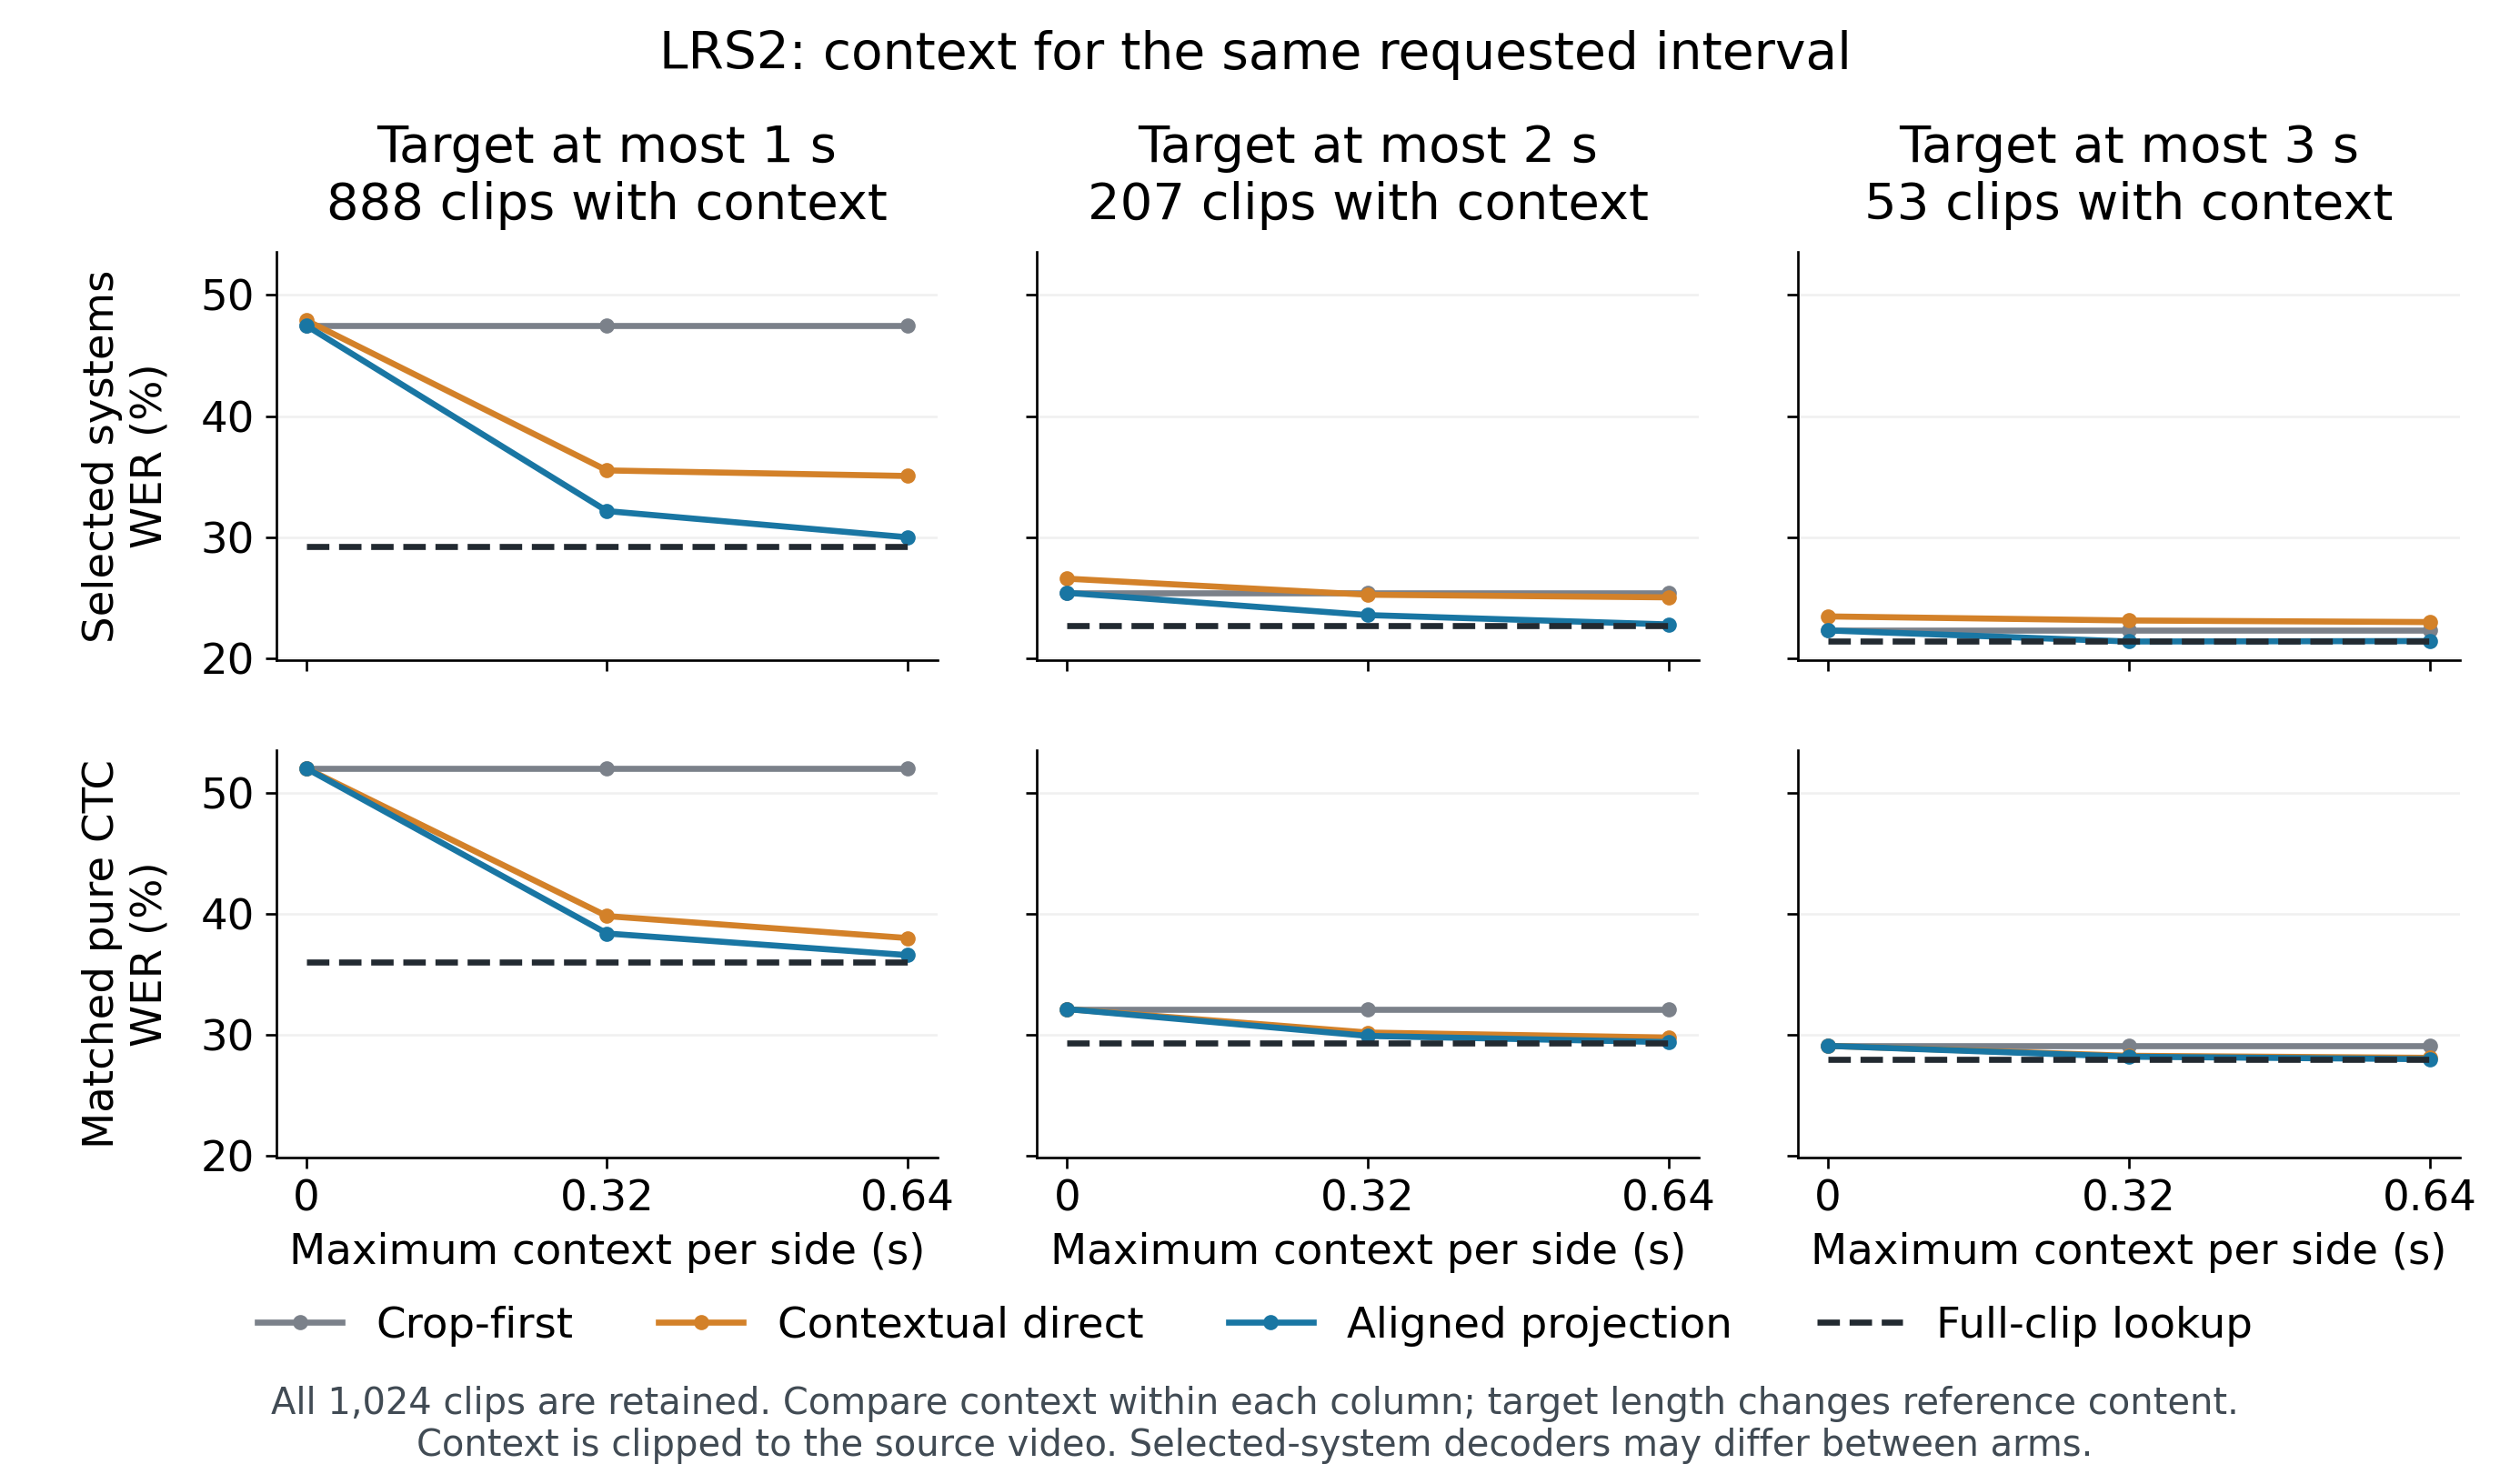
\includegraphics[width=\linewidth]{fig_EN_B1_Context_Grid.png}
 \caption{LRS2 duration experiment on 1,024 clips. Compare context budgets
 within a column: the target text is fixed there. Columns change the requested
 content and are not competing estimates of the same transcript. Both
 development-selected systems and matched pure CTC are shown.}
 \label{fig:english-context}
\end{figure}
The one-second LRS2 target provides a substantial context opportunity
(Figure~\ref{fig:english-context}). Selected projection decreases from
\EnglishOneNoContext{}\% without context to 32.151\% at a 0.32-second
per-side allowance and \EnglishOneContext{}\% at 0.64 seconds. At the latter
budget, contextual direct is 35.049\%. Under matched pure CTC, direct and
projection are 37.974\% and 36.566\%, a 1.408-point reduction with pointwise
source-bootstrap interval [1.023, 1.819] when expressed as an improvement.

The opportunity shrinks as the target covers more of these short clips.
Outside context exists for 888 of 1,024 clips at a one-second target,
207 at two seconds, and only 53 at three seconds. With a one-second target
and a nominal 0.64-second per-side budget, mean actual input is 1.526 seconds;
mean total added context is 0.541 seconds.

The complete VLR grid provides a different duration distribution
(Appendix~\ref{app:duration}). Outside context exists for 1,022 clips at
one- and two-second targets, and 1,012 at three seconds. With greedy decoding,
one-second crop-first WER is 82.659\%, contextual direct with the larger
budget is 57.018\%, and projection is 56.490\%. Its 0.529-point advantage
over direct has pointwise interval [0.222, 0.847] when expressed as a reduction.
Pure CTC gives a corresponding 0.608-point reduction [0.230, 0.996].
At two- and three-second targets, the incremental greedy C--B differences
are -0.053 and -0.044 points, with intervals including zero. Duration therefore
affects both the availability of outside evidence and the benefit of retaining
context through decoding. Context budgets are compared within a fixed target;
different target lengths request different text.

The Spanish and ViCocktail grids extend this comparison to different
corpus/model conditions (Appendix~\ref{app:duration}). At the 0.64-second
allowance, selected Spanish projection changes from 105.737\% to 87.330\%
for the one-second target, and from 89.499\% to 79.991\% for two seconds.
Under matched pure CTC, its improvements over contextual direct are
2.270, 1.558, and 0.830 points for one-, two-, and three-second targets;
the corresponding pointwise intervals all favor projection.
ViCocktail shows a different readout profile. Selected projection improves
from 70.109\% to 59.447\% for one-second requests, but the matched pure-CTC
C--B difference is +0.067 points with interval [-0.153, +0.308]. At two and
three seconds, the matched reductions are 0.133 and 0.102 points. A sizable
context gain can therefore coexist with little additional projection gain.

Increasing context beyond 0.32 seconds also has a corpus-dependent return.
On one-second targets with outside context, the matched-CTC change from
0.32 to 0.64 seconds per side is -3.574 points on VLR, -2.064 on LRS2,
-0.585 on Spanish, and -2.345 on ViCocktail. The Spanish interval includes
zero, whereas the other three favor the larger budget. These paired results
support evaluating context budgets for the intended request and recognizer;
they do not establish an adaptive policy or a universal optimal budget.

\subsection{Whole-transcript recognition favors full input}
\begin{table}[tb]
\centering\small
\caption{Whole-transcript WER (\%) under matched pure CTC, 512 clips per corpus. The shared sliding schedule partitions each clip into balanced targets of at most two seconds with 0.64 s context per side. Full-clip output uses the same reference transcript. Intervals are pointwise source-bootstrap intervals.}
\label{tab:whole}
\resizebox{\textwidth}{!}{%
\begin{tabular}{lrrrl}
\toprule
Corpus & Direct sliding & Projected sliding & Full clip & C--F (pp) \\
\midrule
VLR & 48.667 & 48.452 & 42.877 & +5.575 [+4.641, +6.491] \\
LRS2 & 28.936 & 28.186 & 27.286 & +0.900 [+0.158, +1.631] \\
Spanish & 78.866 & 77.353 & 74.558 & +2.795 [+1.622, +4.239] \\
ViCocktail & 47.723 & 47.691 & 43.756 & +3.935 [+3.066, +4.743] \\
\bottomrule
\end{tabular}%
}
\end{table}

Projected sliding can improve direct sliding, but full-clip recognition
remains stronger on the same complete transcripts
(Table~\ref{tab:whole}). Joining contextual target CTC scores and decoding
once removes some concatenation errors without closing that gap.
At the two-second schedule, this control removes 25, 0, 2, and 10 errors
relative to projected pure-CTC sliding on VLR, LRS2, Spanish, and ViCocktail.

The error balance varies across corpora. Under matched CTC, projected sliding
relative to full-clip decoding
adds 431 substitutions and 589 insertions on VLR while reducing deletions
by 451; Spanish instead adds 220 deletions and 20 substitutions while reducing
insertions by 33. These different error balances are compatible with disruption
of recognition and repeated local decisions, extending beyond duplicated text
at window seams.

\subsection{Query workload determines the cost advantage}
\begin{table}[tb]
\centering\small
\caption{Matched pure-CTC response cost on 32 stratified calibration clips per corpus. Values are across-clip medians after reducing three fresh sessions to one median per clip. All arms use beam 40 with token pruning 64 on the same GTX 1650 Ti. The final column counts paired clips on which C is faster than F. Short clips can deduplicate requests; these descriptive timings do not measure assessment accuracy.}
\label{tab:matched-query-cost}
\begin{tabular}{lrrrrrr}
\toprule
Corpus & Queries & A (s) & B (s) & C (s) & F (s) & C $<$ F \\
\midrule
VLR & 1 & 0.390 & 0.432 & 0.623 & 1.221 & 28/32 \\
VLR & 3 & 1.159 & 1.269 & 1.658 & 1.034 & 2/32 \\
VLR & 5 & 1.954 & 2.128 & 2.865 & 1.093 & 0/32 \\
LRS2 & 1 & 0.338 & 0.362 & 0.441 & 0.455 & 22/32 \\
LRS2 & 3 & 1.026 & 0.979 & 0.459 & 0.431 & 6/32 \\
LRS2 & 5 & 1.681 & 1.599 & 0.561 & 0.462 & 6/32 \\
Spanish & 1 & 0.378 & 0.419 & 0.589 & 0.987 & 29/32 \\
Spanish & 3 & 1.149 & 1.227 & 1.584 & 0.989 & 9/32 \\
Spanish & 5 & 1.903 & 2.037 & 2.785 & 1.014 & 0/32 \\
ViCocktail & 1 & 0.350 & 0.383 & 0.552 & 0.677 & 28/32 \\
ViCocktail & 3 & 1.033 & 1.132 & 1.458 & 0.741 & 10/32 \\
ViCocktail & 5 & 1.734 & 1.909 & 2.563 & 0.708 & 5/32 \\
\bottomrule
\end{tabular}
\end{table}

Holding the decoder fixed reveals a consistent workload distinction
(Table~\ref{tab:matched-query-cost}). For one request, projection is faster
than fresh full-clip lookup on 28/32 VLR clips, 22/32 LRS2 clips, 29/32
Spanish clips, and 28/32 ViCocktail clips. Their paired median C--F time
differences are $-0.612$, $-0.027$, $-0.378$, and $-0.083$ seconds.
For five requested intervals, the paired differences become $+1.698$,
$+0.105$, $+1.824$, and $+0.938$ seconds. Full-clip recognition pays its
initial cost once and reuses the resulting transcript and temporal index.
Marginal medians in the table and medians of paired differences describe
different summaries; they need not differ by the same amount.

Projection also has a cost relative to contextual direct decoding. The paired
median C--B difference is positive in all twelve corpus/workload cells,
ranging from 0.017 to 0.754 seconds. Encoding frame counts are identical
between B and C in every paired clip. C generally decodes a longer sequence
and adds alignment, but distinct targets can sometimes share a contextual
prediction. In LRS2, this reuse reduces C's decode count relative to B on
seven clips with three requests and eight with five; C is faster on each of
those clips. This is the cache behavior described in
Section~\ref{sec:query-computation}, not an additional accuracy gain.

The supplement reports selected-system costs, matched tail latency, and memory.
Together with the paired accuracy results, these measurements distinguish the
cost of a bounded request from the benefit of amortizing full-clip recognition
over a session.

\section{Discussion}

\subsection{Separating recognition support from the requested answer}
The central result is that an output boundary need not be an input boundary.
Keeping neighboring visual evidence improves recognition of a fixed request,
and the real-versus-padding intervention shows that this evidence supplies more
than additional frames. The interval formulation makes that distinction usable
with existing recognizers: context is admitted at encoding, while output scope
can be enforced at the state or transcript level.

The matched comparisons locate the value of projection more precisely.
Contextual direct decoding captures most of the benefit of admitting context.
Projection adds a smaller improvement at the principal operating point in all
four corpora, with more substantial effects in several short-target conditions.
The LRS2 availability analysis shows why an aggregate over short clips can
understate this opportunity: most two-second requests already cover the whole
clip. Together with the decoder screen, the results support treating readout as
a design decision conditioned on the recognizer and request, rather than using
one output rule for every operating point.

\subsection{Practical use and computational reuse}
The intended application is passage-level visual transcription: an editor or
viewer selects a time span and receives the words assigned to it, with a visible
allowance for surrounding video. This is useful when visual input is the
available speech signal and the full transcript has not already been computed.
The present evidence measures recognition and computational cost; a user study
would be needed to quantify editing-time or accessibility benefits.

Two workload regimes follow from the measurements. An isolated request can
benefit from processing a bounded passage; repeated requests can amortize a
full-clip transcript and temporal index. Full-clip recognition also remains
stronger for complete transcripts. Within bounded processing, direct readout
offers the lower measured median cost, while projection trades additional
decoding and alignment for its accuracy benefit. These operating distinctions
give applications a concrete basis for selecting an inference strategy.

\subsection{Scope of the evidence}
Word timing is automatic. The tested reference perturbations preserve the
favorable C--A and C--B point-difference signs, including matched decoders,
but fine allocation is more sensitive: a \(+160\) ms shift makes uniform-word
allocation better than aligned projection by 1.041 points on VLR and 0.245 on
LRS2. Independent review of boundary words would clarify this finer comparison.
The four corpus/model settings also differ in duration, training history, and
source diversity; Spanish has 12 recording sources and high absolute error.
The assessment material was available in earlier research. Results therefore
support the stated within-corpus comparisons, with prospective source-held
replication and evaluation outside the present recognizer family as valuable
extensions. The cost measurements characterize a stratified local-GPU sample.

\subsection{Toward request-dependent computation}
The next methodological question is whether observable request geometry and
predictive uncertainty can select context or readout more efficiently than a
fixed strategy. Such a policy should be developed on separate sources and
evaluated against fixed context budgets, contextual direct, projection, and
cached full-clip lookup under compatible input permissions. Its feature
extraction and routing costs must be included. The current duration and workload
results provide the empirical basis for this question; they are not an
evaluation of an adaptive policy.

\section{Conclusion}
Context-aware interval transcription separates the evidence used to recognize
speech from the span of text requested by the user. Prediction-aligned projection
implements this separation using a pretrained visual recognizer and its native
CTC scores. Four-corpus experiments show improved requested-interval recognition
over input cropping, while matched decoders distinguish contextual encoding
from the incremental effect of transcript projection. Context availability and
computational reuse explain the practical operating conditions. This formulation
extends pretrained VSR to selective passage requests and provides an empirical
basis for balancing context, readout, and work across queries.


\begingroup
\small
\bibliographystyle{elsarticle-harv}
\bibliography{references}
\endgroup

\clearpage
\appendix
\section{Corpus geometry and source weighting}
\label{app:corpus}
\begin{table}[tb]
\centering\small
\caption{Geometry and source concentration of the principal E1 cohorts. Mean and median describe prepared clip duration. No context means the at-most-two-second target covers the clip. Added is the mean total observed context across both sides under the frozen placement rule. Max. source is the largest recording source's share of target reference units.}
\label{tab:corpus-inventory}
\resizebox{\textwidth}{!}{%
\begin{tabular}{lrlrrr}
\toprule
Corpus & Mean (s) & Median [IQR] (s) & No context (\%) & Added (s) & Max. source (\%) \\
\midrule
VLR & 5.782 & 5.64 [4.96, 6.44] & 0.2 & 0.851 & 4.8 \\
LRS2 & 1.642 & 1.44 [1.16, 1.92] & 79.3 & 0.099 & 3.2 \\
Spanish & 5.913 & 4.30 [2.16, 7.79] & 23.2 & 0.596 & 24.9 \\
ViCocktail & 5.830 & 5.16 [4.24, 7.00] & 0.9 & 0.843 & 13.4 \\
\bottomrule
\end{tabular}%
}
\end{table}

\begin{table}[tb]
\centering\small
\caption{Ranges after omitting one recording source at a time from the principal selected-system comparison. These are descriptive source-influence ranges, not confidence intervals. The primary source-bootstrap uncertainty remains in Table~\ref{tab:primary-intervals}.}
\label{tab:source-influence}
\begin{tabular}{lll}
\toprule
Corpus & C--A range (pp) & C--B range (pp) \\
\midrule
VLR & [-8.278, -7.990] & [-0.152, -0.139] \\
LRS2 & [-2.421, -2.226] & [-1.962, -1.784] \\
Spanish & [-5.604, -4.969] & [-1.751, -1.111] \\
ViCocktail & [-3.919, -3.370] & [-1.210, -0.833] \\
\bottomrule
\end{tabular}
\end{table}

The duration statistics in Table~\ref{tab:corpus-inventory} describe the exact
principal assessment cohorts, measured from prepared frames at 25 fps. They
are not estimates of the complete source datasets. The interval in the median
column gives the 25th and 75th percentiles. For the two-second request, 79.3\%
of LRS2 clips already fit inside the target, compared with 0.2\% on VLR,
23.2\% on Spanish, and 0.9\% on ViCocktail. The principal hash-based start,
center and end placements further limit which margin is available. Mean
observed context is therefore smaller than the maximum 1.28 seconds across
both sides, even in corpora with substantially longer clips.

Recording sources also have different weights. The largest Spanish source
contributes 24.9\% of the target reference units, compared with 4.8\% for VLR,
3.2\% for LRS2 and 13.4\% for ViCocktail. Both principal point differences
remain favorable to projection after omitting any single source
(Table~\ref{tab:source-influence}). These descriptive ranges address the
influence of one recording; they do not imply significance or replace the
source-bootstrap intervals. In particular, the adjusted Spanish C--B
interval still includes zero. Duration, recording composition and checkpoint
history should consequently accompany any interpretation across corpora.

\subsection{Recognition by actual context availability}
\label{app:availability}
\begin{table}[tb]
\centering\footnotesize
\setlength{\tabcolsep}{4pt}
\caption{Post-hoc context-availability analysis of the frozen principal assessment,
with the same pure-CTC decoder for A/B/C. WER is in percent; C--B differences
are in percentage points with explanatory pointwise 95\% paired-source
intervals, without multiplicity adjustment. Every clip is retained.
Availability groups follow the fixed request geometry and are descriptive.}
\label{tab:context-availability}
\begin{tabular}{llrrrrl}
\toprule
Corpus & Context & Clips & A & B & C & C--B [95\% CI] \\
\midrule
VLR & None & 27 & 89.195 & 89.195 & 89.195 & +0.000 [+0.000, +0.000] \\
VLR & Left & 3,791 & 59.678 & 47.809 & 47.626 & -0.183 [-0.242, -0.124] \\
VLR & Right & 3,717 & 55.839 & 55.078 & 54.901 & -0.177 [-0.242, -0.107] \\
VLR & Both & 3,771 & 61.056 & 48.816 & 48.658 & -0.158 [-0.229, -0.087] \\
LRS2 & None & 986 & 29.836 & 29.836 & 29.836 & +0.000 [+0.000, +0.000] \\
LRS2 & Left & 83 & 33.673 & 25.510 & 24.490 & -1.020 [-1.944, -0.208] \\
LRS2 & Right & 96 & 27.014 & 23.381 & 22.275 & -1.106 [-2.070, -0.312] \\
LRS2 & Both & 78 & 34.836 & 26.230 & 24.795 & -1.434 [-2.740, -0.405] \\
Spanish & None & 217 & 84.358 & 84.358 & 84.358 & +0.000 [+0.000, +0.000] \\
Spanish & Left & 234 & 81.993 & 78.727 & 77.722 & -1.005 [-2.003, -0.472] \\
Spanish & Right & 260 & 81.271 & 80.146 & 79.351 & -0.794 [-1.366, -0.276] \\
Spanish & Both & 223 & 86.188 & 84.933 & 83.049 & -1.883 [-2.902, -1.174] \\
ViCocktail & None & 11 & 59.649 & 59.649 & 59.649 & +0.000 [+0.000, +0.000] \\
ViCocktail & Left & 361 & 54.862 & 53.120 & 52.980 & -0.139 [-0.277, -0.034] \\
ViCocktail & Right & 407 & 52.642 & 50.605 & 50.385 & -0.220 [-0.369, -0.083] \\
ViCocktail & Both & 388 & 58.996 & 54.204 & 54.089 & -0.115 [-0.382, +0.181] \\
\bottomrule
\end{tabular}
\end{table}

Table~\ref{tab:context-availability} separates the principal assessment by
whether the recorded input adds left, right, both, or no context to the target.
It uses matched pure CTC throughout. With no outside context, A/B/C return
identical predictions on all 27 VLR, 986 LRS2, 217 Spanish, and 11 ViCocktail
clips. The whole-cohort difference therefore combines an identity subset with
clips on which contextual inference can change the result.

The three LRS2 outside-context groups show C--B reductions of 1.020--1.434
points. VLR's corresponding reductions are 0.158--0.183 points, and Spanish's
are 0.794--1.883 points. ViCocktail shows smaller differences, with the interval
for its both-context group including zero. This decomposition complements the
duration experiment without excluding short clips from the principal endpoint.
The groups differ in target position and clip duration; comparisons across
groups are descriptive rather than controlled left-versus-right interventions.

\section{Primary comparison uncertainty}
\begin{table}[tb]
\centering\small
\caption{Paired source-bootstrap intervals for the eight primary system comparisons. Negative differences favor projection. Bonferroni adjustment uses 99.375\% individual percentile intervals from 10,000 draws; coverage is approximate.}
\label{tab:primary-intervals}
\begin{tabular}{lll}
\toprule
Corpus & Contrast & Difference and family-adjusted interval (pp) \\
\midrule
VLR & C--A & -8.168 [-9.086, -7.282] \\
VLR & C--B & -0.145 [-0.194, -0.097] \\
LRS2 & C--A & -2.366 [-3.377, -1.449] \\
LRS2 & C--B & -1.876 [-2.916, -0.852] \\
Spanish & C--A & -5.281 [-7.487, -3.903] \\
Spanish & C--B & -1.357 [-3.025, +0.020] \\
ViCocktail & C--A & -3.574 [-5.126, -2.001] \\
ViCocktail & C--B & -0.986 [-1.834, -0.183] \\
\bottomrule
\end{tabular}
\end{table}

Table~\ref{tab:primary-intervals} reports the complete primary family. Source
resampling preserves paired arm predictions within each sampled recording.
It addresses within-source dependence more directly than treating every
clip as independent, but it cannot account for unobserved dependence between
recordings or repair prior exposure to the assessment corpus. In particular,
the Spanish C--B interval includes zero after the family adjustment.

\section{Complete duration grids and actual context}
\label{app:duration}
\begingroup
\footnotesize
\setlength{\tabcolsep}{3pt}
\begin{longtable}{lrrrrrr}
\caption{Complete duration grids: development-selected WER (\%). Cohort sizes are VLR: 1,024; LRS2: 1,024; Spanish: 934; ViCocktail: 1,024. Target length and per-side context are maxima clipped to available video. Compare context within a fixed target; target length changes reference content. Decoders: VLR A/B/C: greedy/greedy/greedy; LRS2 A/B/C: hybrid10/hybrid50/hybrid10; Spanish A/B/C: hybrid10/hybrid50/hybrid10; ViCocktail A/B/C: hybrid10/hybrid50/hybrid10.}\label{tab:duration-grid}\\
\toprule
Corpus & Target (s) & Context (s) & Units & A & B & C \\
\midrule
\endfirsthead
\toprule
Corpus & Target (s) & Context (s) & Units & A & B & C \\
\midrule
\endhead
\midrule
\multicolumn{7}{r}{Continued on the next page}\\
\endfoot
\bottomrule
\endlastfoot
VLR & 1 & 0 & 3783 & 82.659 & 82.659 & 82.659 \\
VLR & 1 & 0.32 & 3783 & 82.659 & 60.455 & 60.005 \\
VLR & 1 & 0.64 & 3783 & 82.659 & 57.018 & 56.490 \\
VLR & 2 & 0 & 7608 & 59.727 & 59.727 & 59.727 \\
VLR & 2 & 0.32 & 7608 & 59.727 & 49.882 & 49.724 \\
VLR & 2 & 0.64 & 7608 & 59.727 & 48.686 & 48.633 \\
VLR & 3 & 0 & 11449 & 50.808 & 50.808 & 50.808 \\
VLR & 3 & 0.32 & 11449 & 50.808 & 46.161 & 46.161 \\
VLR & 3 & 0.64 & 11449 & 50.808 & 45.061 & 45.017 \\
LRS2 & 1 & 0 & 3692 & 47.481 & 47.914 & 47.481 \\
LRS2 & 1 & 0.32 & 3692 & 47.481 & 35.509 & 32.151 \\
LRS2 & 1 & 0.64 & 3692 & 47.481 & 35.049 & 29.984 \\
LRS2 & 2 & 0 & 5052 & 25.396 & 26.564 & 25.396 \\
LRS2 & 2 & 0.32 & 5052 & 25.396 & 25.238 & 23.555 \\
LRS2 & 2 & 0.64 & 5052 & 25.396 & 25.020 & 22.783 \\
LRS2 & 3 & 0 & 5353 & 22.287 & 23.445 & 22.287 \\
LRS2 & 3 & 0.32 & 5353 & 22.287 & 23.109 & 21.371 \\
LRS2 & 3 & 0.64 & 5353 & 22.287 & 22.978 & 21.409 \\
Spanish & 1 & 0 & 2423 & 105.737 & 102.889 & 105.737 \\
Spanish & 1 & 0.32 & 2423 & 105.737 & 92.035 & 92.778 \\
Spanish & 1 & 0.64 & 2423 & 105.737 & 89.889 & 87.330 \\
Spanish & 2 & 0 & 4428 & 89.499 & 89.273 & 89.499 \\
Spanish & 2 & 0.32 & 4428 & 89.499 & 86.134 & 83.424 \\
Spanish & 2 & 0.64 & 4428 & 89.499 & 83.853 & 79.991 \\
Spanish & 3 & 0 & 6143 & 79.993 & 81.605 & 79.993 \\
Spanish & 3 & 0.32 & 6143 & 79.993 & 80.905 & 78.187 \\
Spanish & 3 & 0.64 & 6143 & 79.993 & 81.345 & 77.601 \\
ViCocktail & 1 & 0 & 4483 & 70.109 & 69.708 & 70.109 \\
ViCocktail & 1 & 0.32 & 4483 & 70.109 & 62.614 & 61.923 \\
ViCocktail & 1 & 0.64 & 4483 & 70.109 & 60.228 & 59.447 \\
ViCocktail & 2 & 0 & 9019 & 54.928 & 54.862 & 54.928 \\
ViCocktail & 2 & 0.32 & 9019 & 54.928 & 51.591 & 50.815 \\
ViCocktail & 2 & 0.64 & 9019 & 54.928 & 50.194 & 48.841 \\
ViCocktail & 3 & 0 & 13733 & 49.290 & 49.712 & 49.290 \\
ViCocktail & 3 & 0.32 & 13733 & 49.290 & 46.843 & 46.137 \\
ViCocktail & 3 & 0.64 & 13733 & 49.290 & 46.232 & 45.453 \\
\end{longtable}
\endgroup

\begin{table}[tb]
\centering\small
\caption{Actual input geometry at a maximum of 0.64 s context per side. Context available counts clips with any outside video; both full counts clips with two complete margins. Input and added context are per-clip means, with added context summed across both sides.}
\label{tab:duration-geometry}
\resizebox{\textwidth}{!}{%
\begin{tabular}{lrrrrrr}
\toprule
Corpus & Target (s) & Clips & Context available & Both full & Input (s) & Added (s) \\
\midrule
VLR & 1 & 1024 & 1022 & 1021 & 2.276 & 1.277 \\
VLR & 2 & 1024 & 1022 & 1011 & 3.268 & 1.271 \\
VLR & 3 & 1024 & 1012 & 910 & 4.219 & 1.228 \\
LRS2 & 1 & 1024 & 888 & 150 & 1.526 & 0.541 \\
LRS2 & 2 & 1024 & 207 & 42 & 1.604 & 0.127 \\
LRS2 & 3 & 1024 & 53 & 13 & 1.626 & 0.035 \\
Spanish & 1 & 934 & 857 & 687 & 2.036 & 1.056 \\
Spanish & 2 & 934 & 717 & 580 & 2.712 & 0.886 \\
Spanish & 3 & 934 & 606 & 477 & 3.275 & 0.741 \\
ViCocktail & 1 & 1024 & 1022 & 1012 & 2.272 & 1.272 \\
ViCocktail & 2 & 1024 & 1013 & 1000 & 3.253 & 1.258 \\
ViCocktail & 3 & 1024 & 1002 & 753 & 4.141 & 1.162 \\
\bottomrule
\end{tabular}%
}
\end{table}

\begin{table}[tb]
\centering\small
\caption{Incremental projection effect relative to contextual direct at a maximum of 0.64 s context per side. Negative differences favor projection. Brackets are explanatory 95\% source-cluster bootstrap intervals, not multiplicity-adjusted confirmatory tests. Each contrast compares the same target and cohort.}
\label{tab:duration-projection}
\begin{tabular}{lrll}
\toprule
Corpus & Target (s) & Selected C--B (pp) & Pure CTC C--B (pp) \\
\midrule
VLR & 1 & -0.529 [-0.847, -0.222] & -0.608 [-0.996, -0.230] \\
VLR & 2 & -0.053 [-0.221, +0.108] & -0.118 [-0.281, +0.027] \\
VLR & 3 & -0.044 [-0.104, +0.017] & -0.079 [-0.156, +0.000] \\
LRS2 & 1 & -5.065 [-6.299, -3.849] & -1.408 [-1.819, -1.023] \\
LRS2 & 2 & -2.237 [-3.136, -1.368] & -0.376 [-0.583, -0.191] \\
LRS2 & 3 & -1.569 [-2.325, -0.821] & -0.112 [-0.205, -0.037] \\
Spanish & 1 & -2.559 [-4.405, -0.330] & -2.270 [-3.435, -1.430] \\
Spanish & 2 & -3.862 [-5.241, -2.146] & -1.558 [-2.205, -1.081] \\
Spanish & 3 & -3.744 [-5.054, -2.697] & -0.830 [-1.193, -0.579] \\
ViCocktail & 1 & -0.781 [-1.677, +0.035] & +0.067 [-0.153, +0.308] \\
ViCocktail & 2 & -1.353 [-2.066, -0.690] & -0.133 [-0.248, -0.012] \\
ViCocktail & 3 & -0.779 [-1.137, -0.320] & -0.102 [-0.194, -0.013] \\
\bottomrule
\end{tabular}
\end{table}

\begin{figure}[tb]
 \centering
 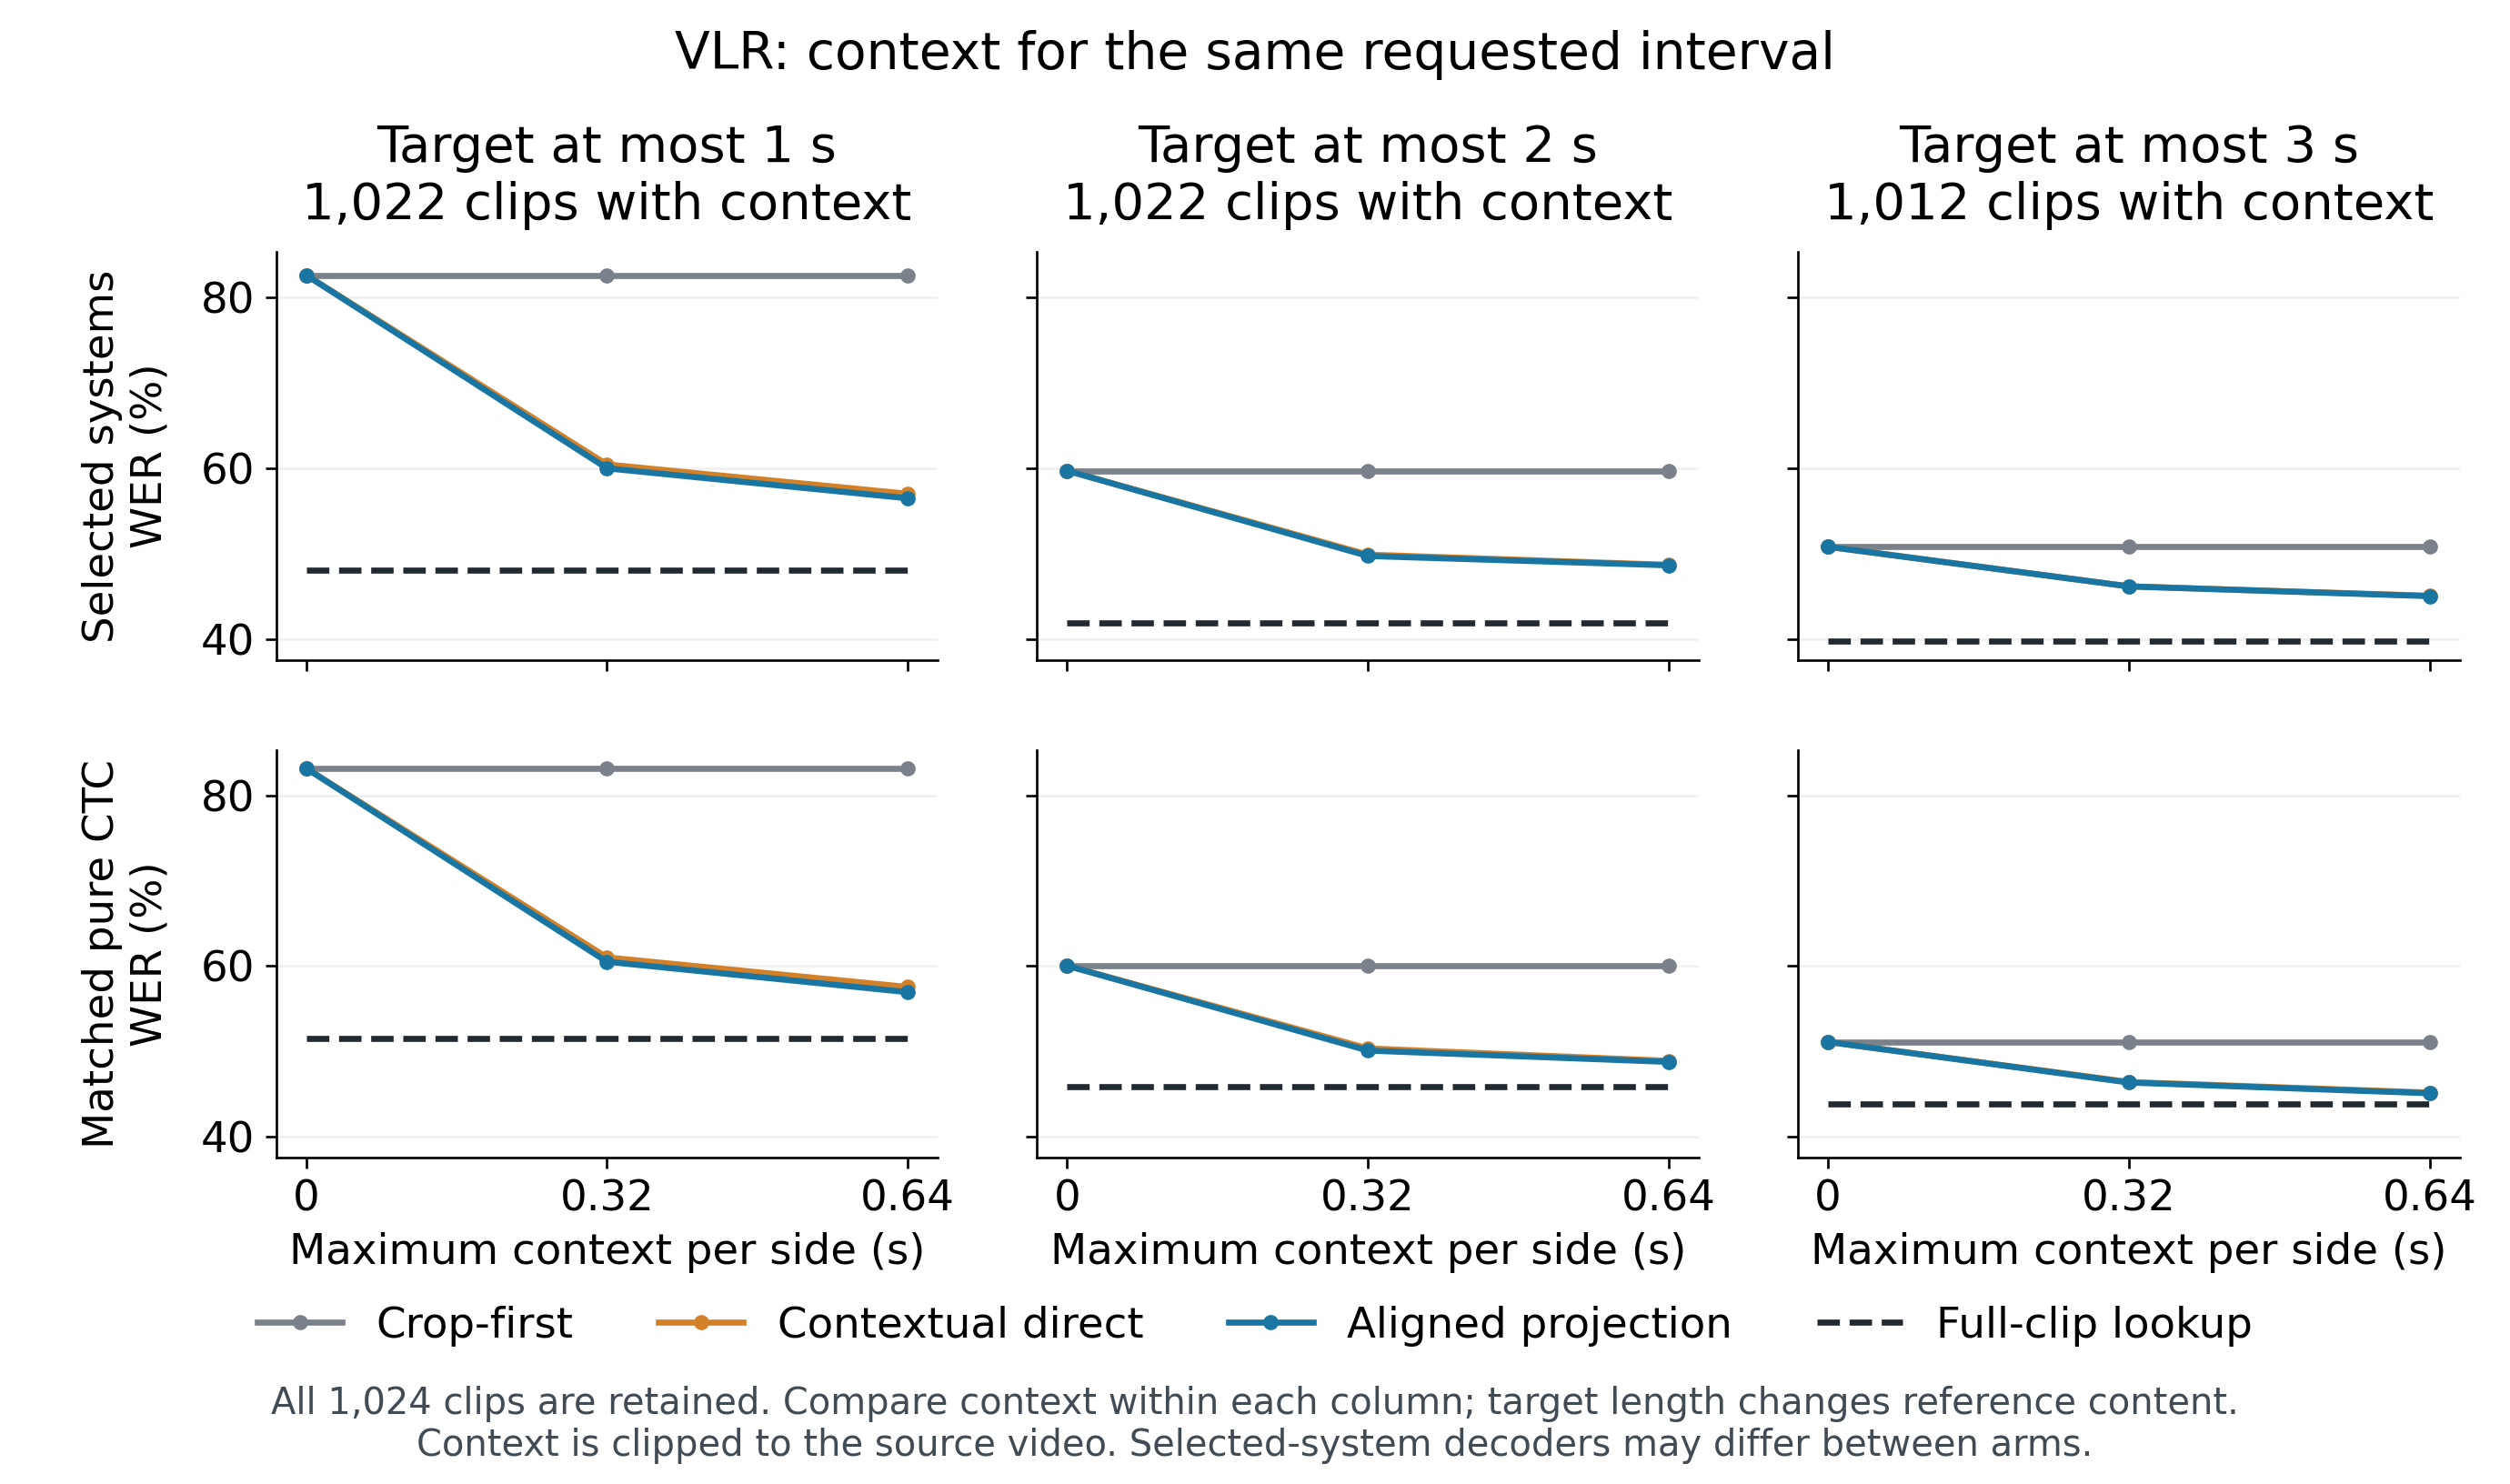
\includegraphics[width=\linewidth]{fig_VLR_T0_Context_Grid.png}
 \caption{VLR duration grid on the complete 1,024-clip cohort. Contextual
 direct and projection are close under the same greedy or pure-CTC decoder.
 The selected full-clip lookup uses a hybrid decoder, so its separation from
 the selected greedy systems includes a decoder difference.}
 \label{fig:vlr-context}
\end{figure}
\begin{figure}[tb]
 \centering
 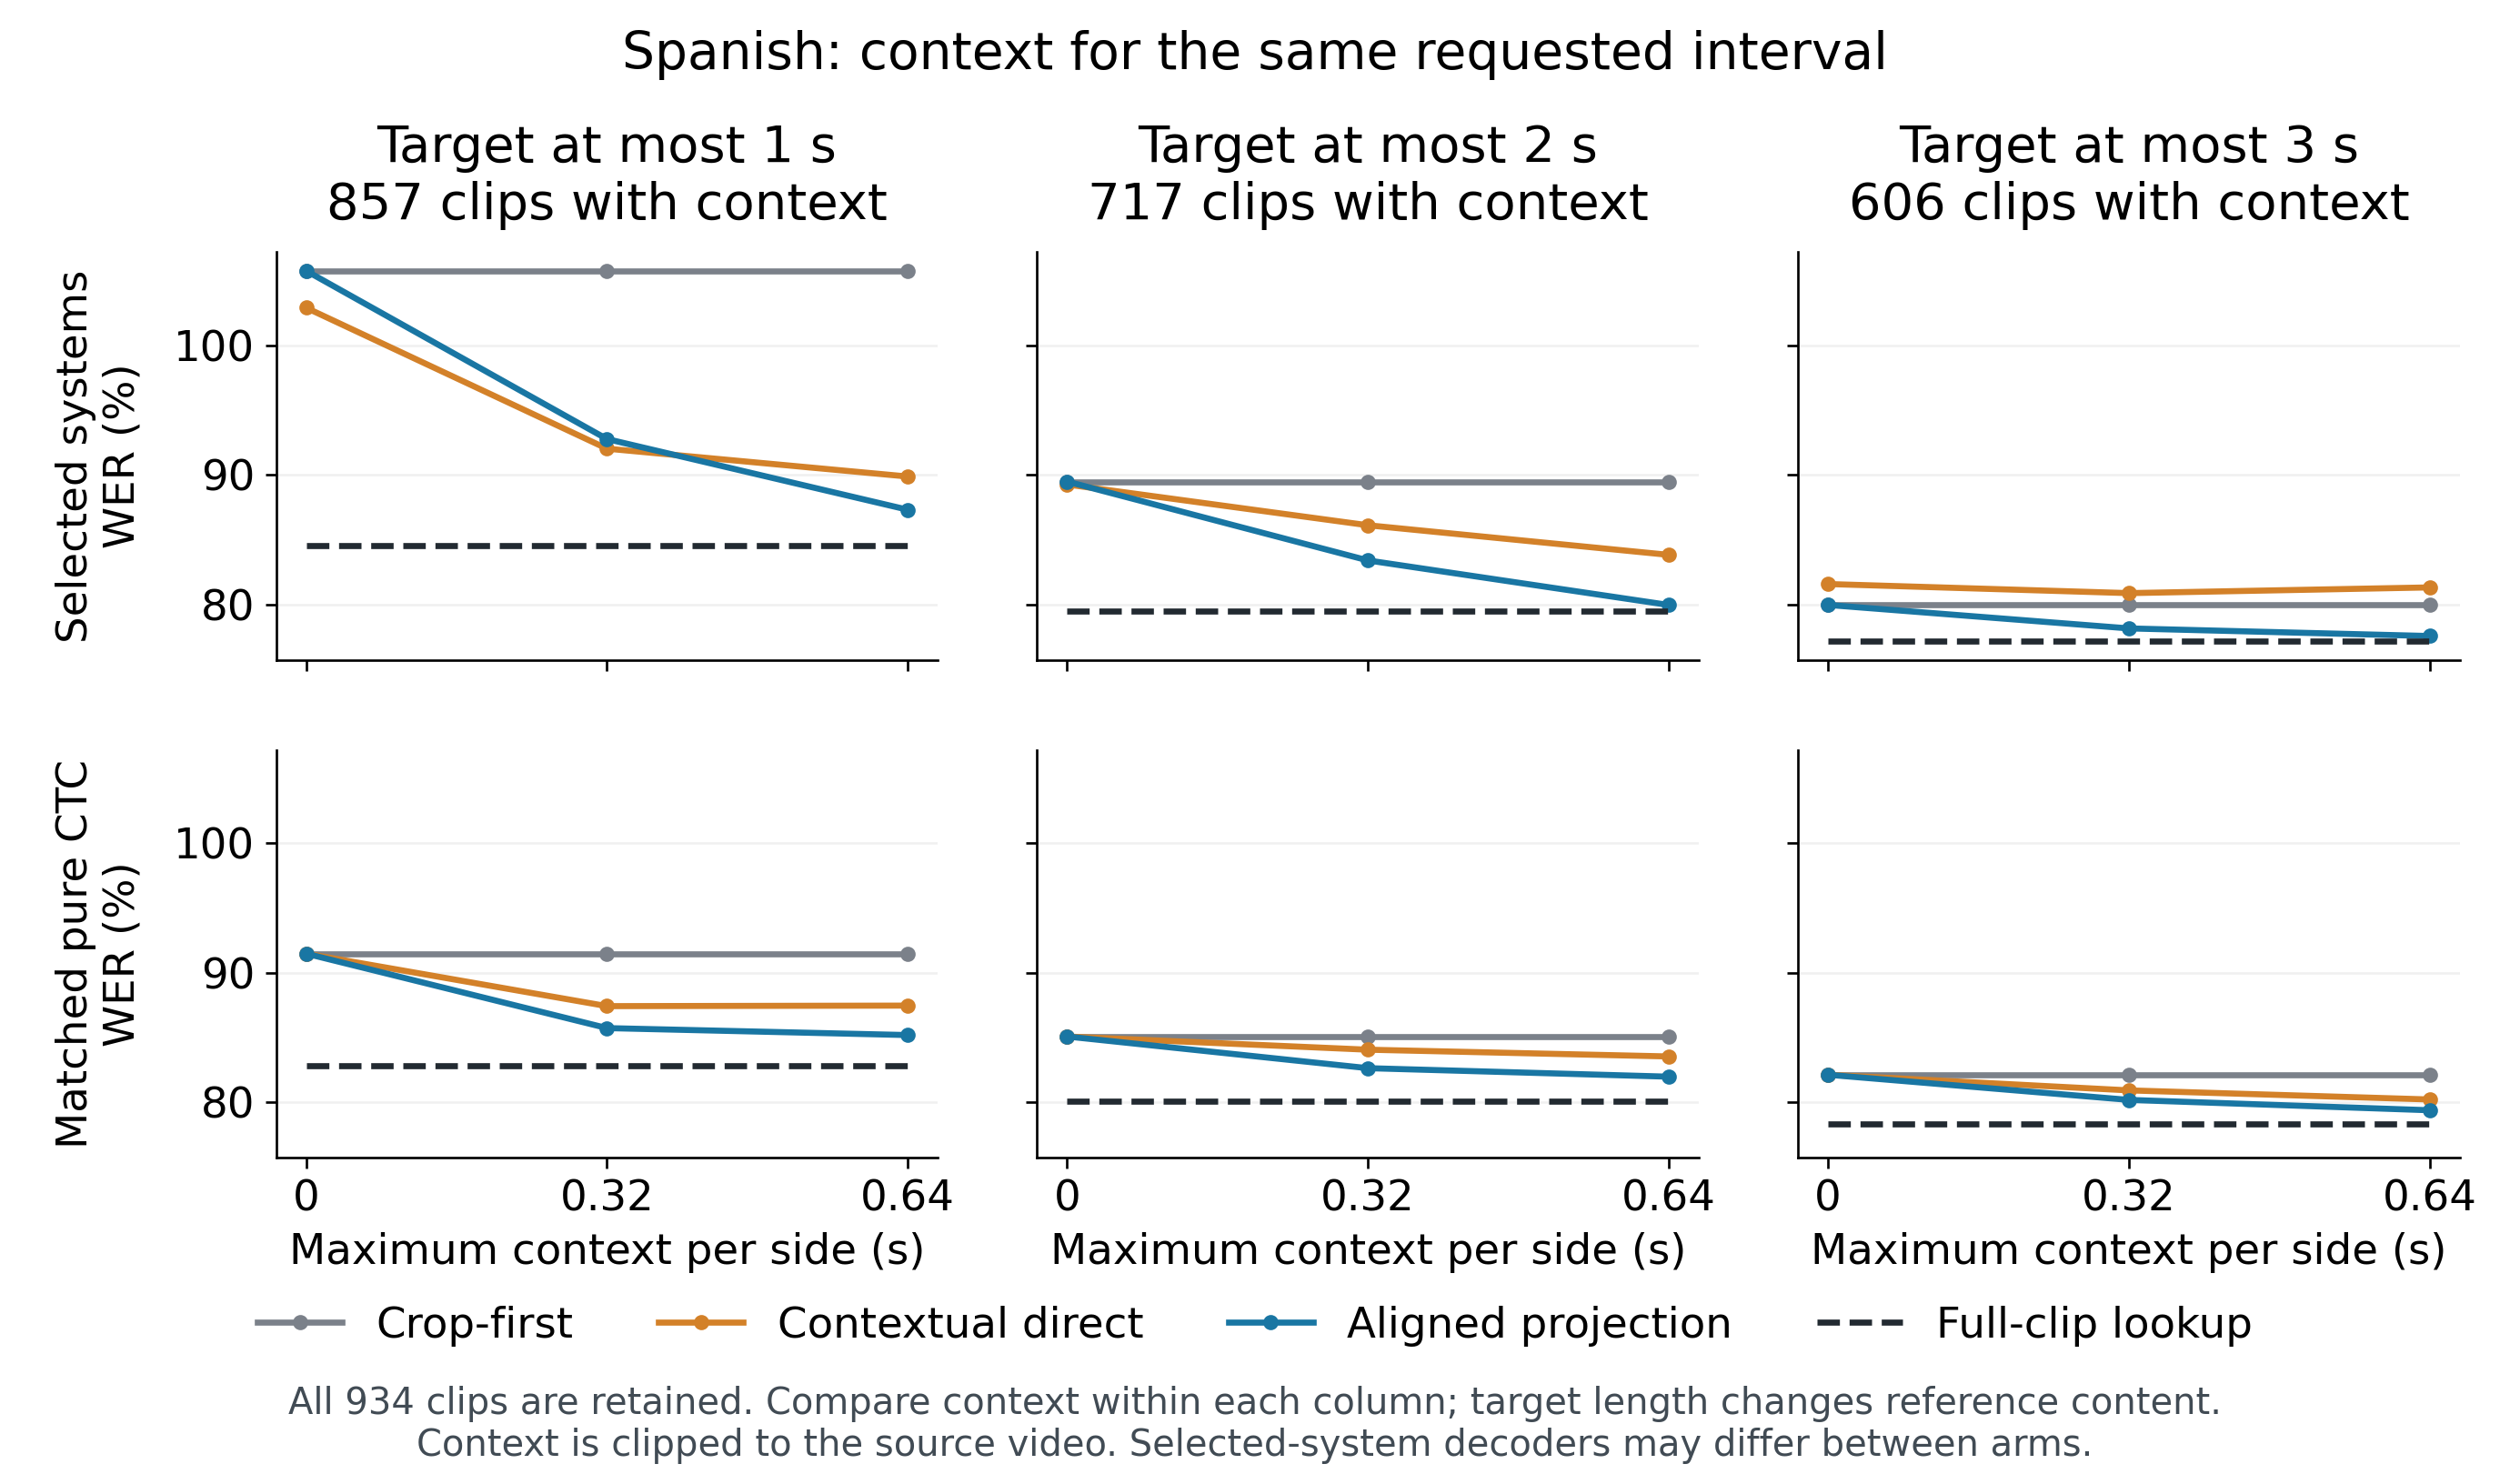
\includegraphics[width=\linewidth]{fig_ES_NATIVE_Context_Grid.png}
 \caption{Spanish duration grid on all 934 eligible clips. Native hybrid
 decoding and pure CTC have different error levels, but both support examining
 context within a fixed target. The same decoder is retained across context
 budgets within each arm. Absolute error remains high on this evaluation cohort.}
 \label{fig:spanish-context}
\end{figure}
\begin{figure}[tb]
 \centering
 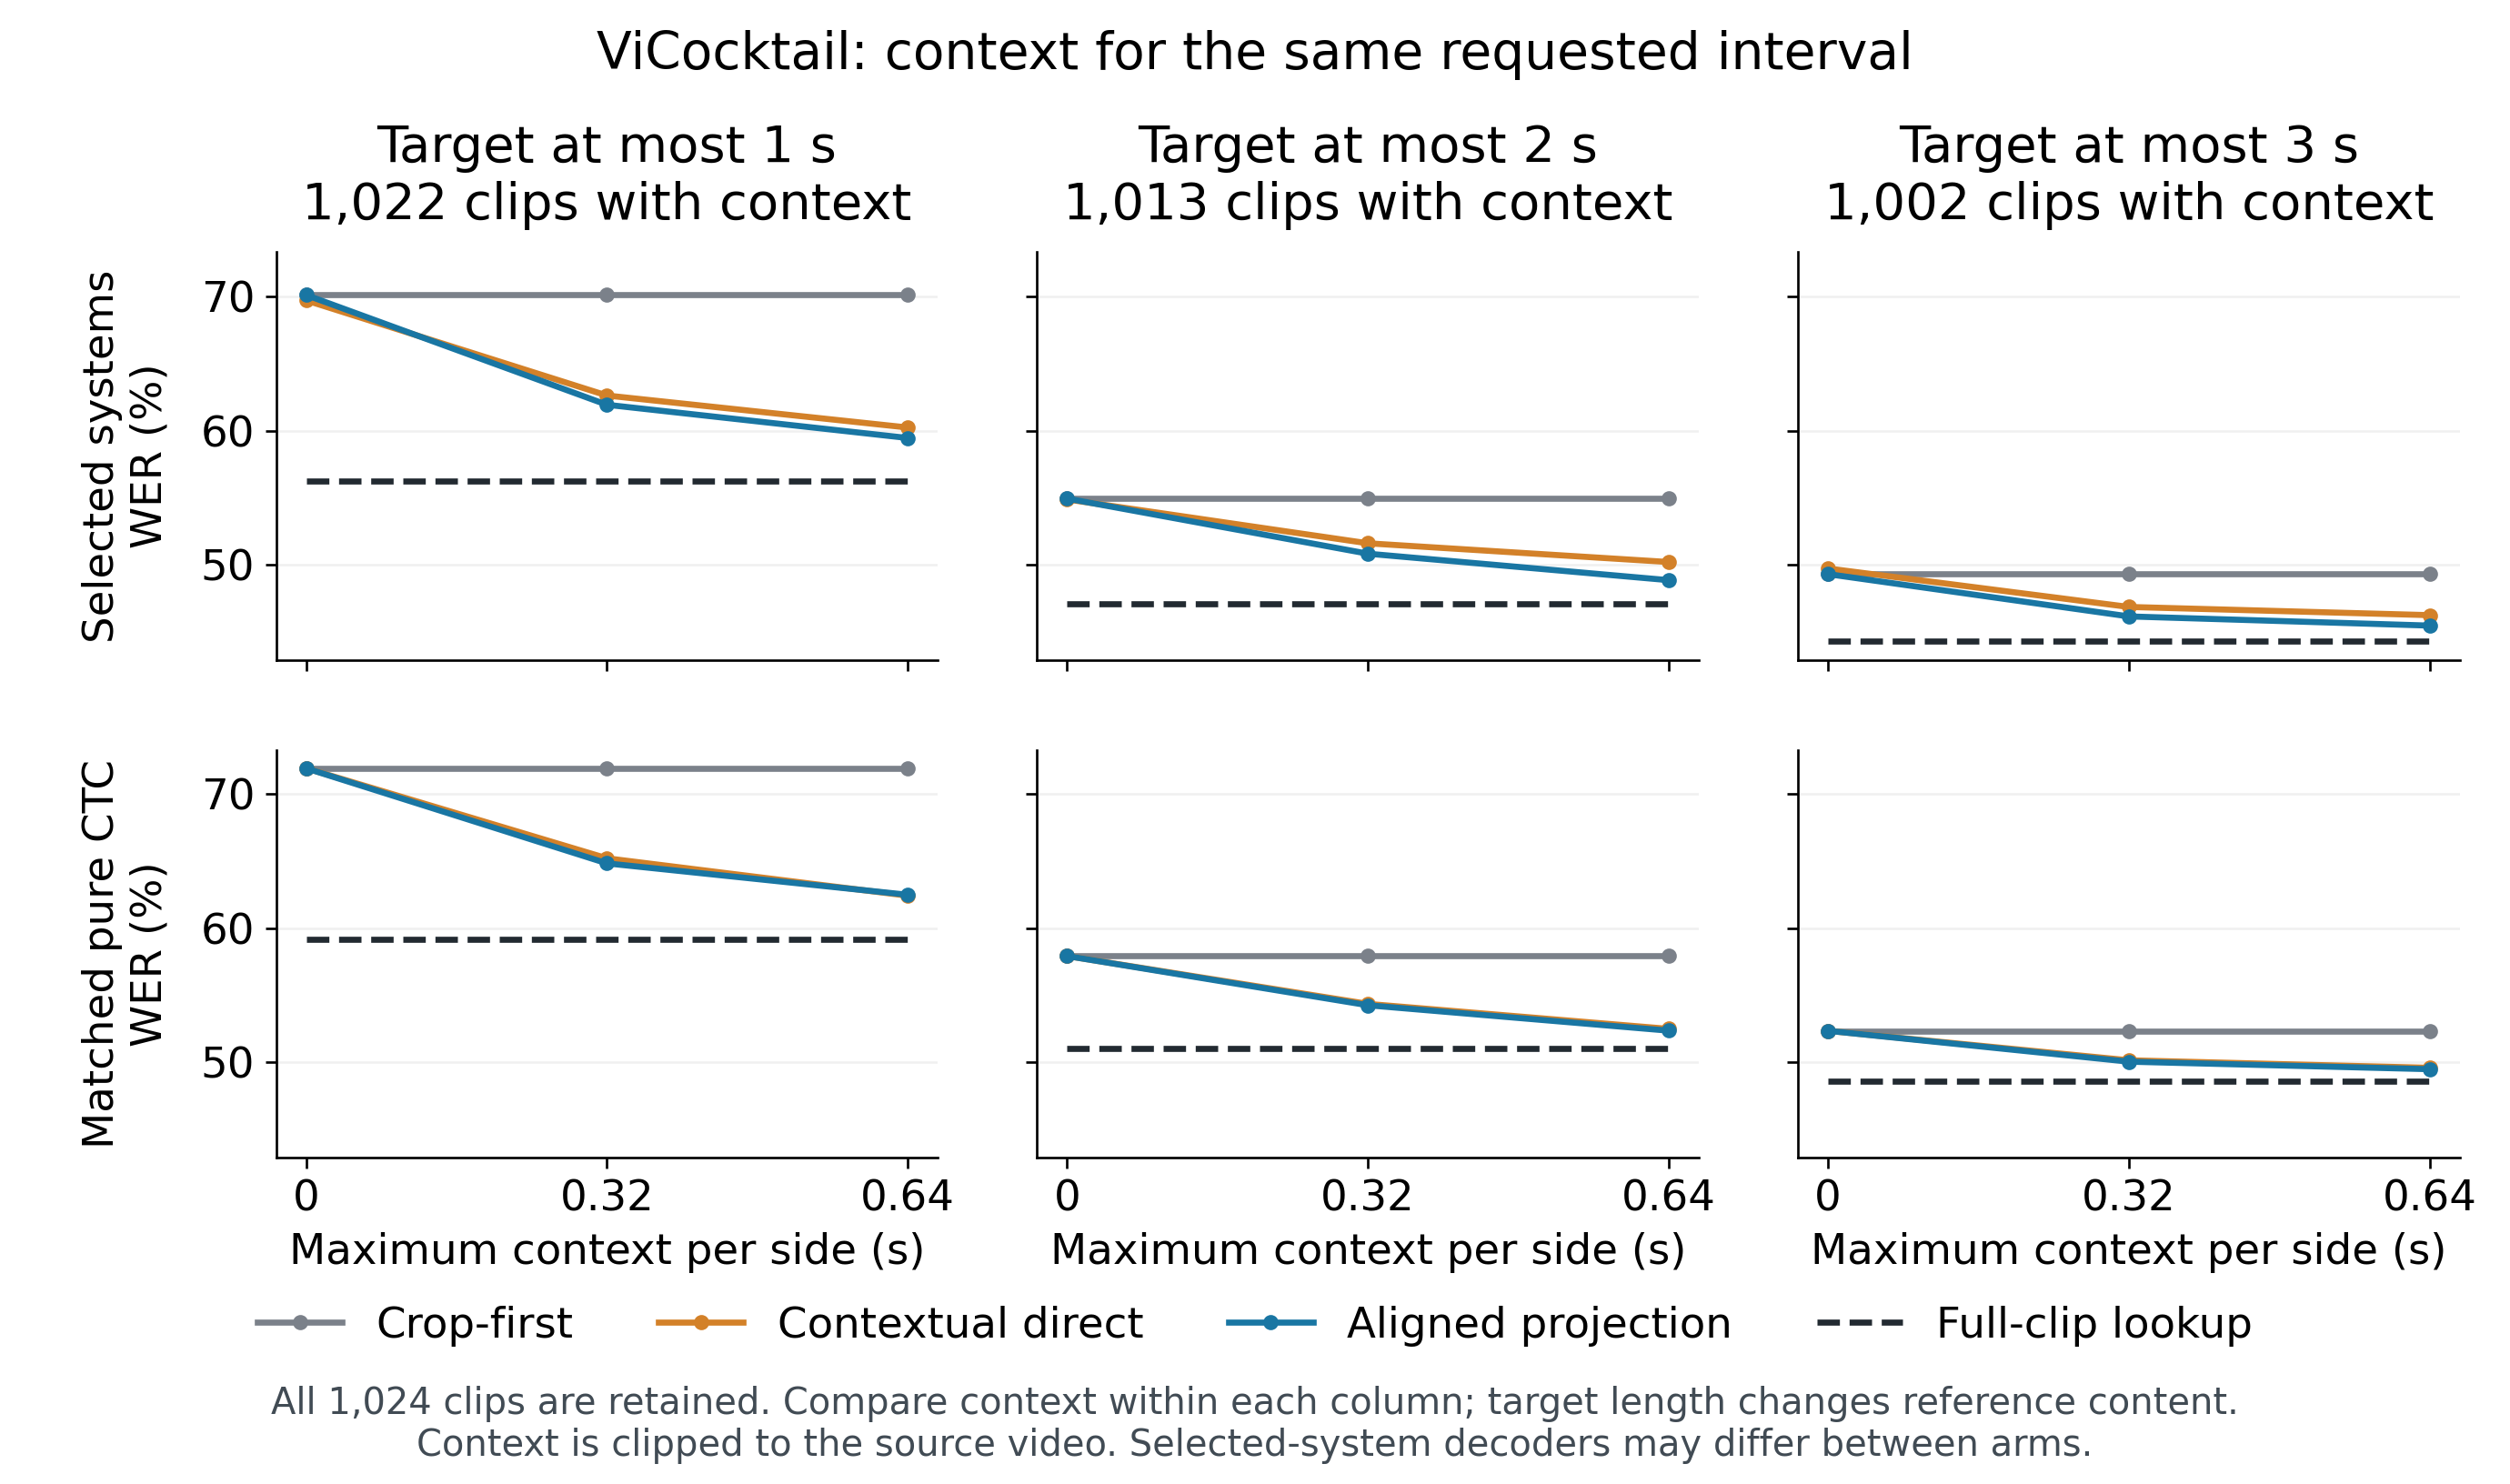
\includegraphics[width=\linewidth]{fig_VC_NATIVE_Context_Grid.png}
 \caption{ViCocktail duration grid on 1,024 clips. Context improves target
 recognition, while matched pure-CTC direct and projected readout remain close.
 The additional selected-system projection gain includes the difference
 between development-selected hybrid weights.}
 \label{fig:vicocktail-context}
\end{figure}
The nominal target and context lengths are converted to 25, 50, or 75 target
frames and 0, 8, or 16 context frames per side. All duration cells use centered
targets, while the principal two-second assessment includes deterministic
start, center, and end placements. Consequently, the duration grid is not an
exact repeat of the principal table even where the nominal lengths coincide.

At zero context, crop-first and projected output agree when the decoder is
the same. This is an identity control, not an additional recognition gain.
The full-clip target baseline is also invariant to the requested context
budget at a fixed target. Table~\ref{tab:duration-geometry} makes clipping
at video boundaries explicit. Clips without outside context remain in every
whole-cohort comparison.

Table~\ref{tab:duration-projection} keeps the incremental C--B comparisons
for every target and corpus. The Spanish matched-CTC reductions span
0.830--2.270 points, whereas the ViCocktail matched differences stay within
0.133 points of zero. The two-second Spanish C--B comparison is stronger in
this centered duration grid than in the principal placement mixture. Different
placement and cohort composition make these complementary comparisons;
the duration result does not replace the principal family-adjusted interval.
Spanish one-second selected WER can exceed 100\% because insertions contribute
to the numerator. The underlying edit counts, rather than a capped percentage,
are retained in every comparison.

\section{Complete context interventions}
\label{app:context-controls}
\begin{table}[tb]
\centering\small
\caption{Complete context interventions: requested-interval WER (\%) on the same clips with outside context within each corpus (VLR 254, LRS2 48, Spanish 202, ViCocktail 254). Targets are centered and at most two seconds. Real, repeat and reverse preserve input length; left/right retain only that margin and therefore change length. Selected A/C use greedy for VLR and hybrid10 otherwise; pure CTC is matched throughout.}
\label{tab:context-controls}
\resizebox{\textwidth}{!}{%
\begin{tabular}{llrrrrrr}
\toprule
Corpus & Regime & Crop A & Real C & Left C & Right C & Repeat C & Reverse C \\
\midrule
VLR & Selected & 60.021 & 50.211 & 51.741 & 57.806 & 54.430 & 55.538 \\
VLR & Pure CTC & 60.549 & 49.947 & 51.688 & 57.753 & 54.378 & 55.643 \\
LRS2 & Selected & 27.508 & 18.123 & 23.948 & 24.272 & 25.890 & 22.330 \\
LRS2 & Pure CTC & 33.333 & 23.625 & 28.479 & 28.479 & 31.068 & 26.861 \\
Spanish & Selected & 84.686 & 70.690 & 76.775 & 81.947 & 80.325 & 78.803 \\
Spanish & Pure CTC & 80.832 & 75.963 & 77.688 & 79.615 & 79.006 & 79.716 \\
ViCocktail & Selected & 57.116 & 50.537 & 54.876 & 54.130 & 59.823 & 60.616 \\
ViCocktail & Pure CTC & 60.429 & 54.550 & 57.210 & 57.163 & 60.616 & 61.223 \\
\bottomrule
\end{tabular}%
}
\end{table}

Table~\ref{tab:context-controls} keeps all five context conditions on the same
outside-context subset in each corpus. Both real margins give lower projected
WER than either margin alone in every displayed setting. The relative value
of the two individual margins is not constant: selected VLR projection gives
51.741\% with the left margin and 57.806\% with the right, whereas ViCocktail
gives 54.876\% and 54.130\%, respectively. Removing a margin also shortens the
encoder input and changes the native output cap, so these differences are
operating-condition comparisons rather than isolated measures of directional
linguistic information. They do not establish a language-specific rule.

Reversing each margin separately preserves its frames and length but changes
their temporal order and continuity with the target. Real context improves
the selected projected output by 5.327 points on VLR, 8.114 on Spanish and
10.079 on ViCocktail, with pointwise intervals excluding zero. LRS2 gives a
4.207-point improvement, but its interval includes zero on the smaller
48-clip subset. The matched pure-CTC contrasts have the same distinction.
Thus repeated-boundary and reversed context probe different properties;
neither intervention alone identifies the source of the recognition benefit.

For the real-versus-repeat contrast, omitting any one recording source keeps
the point difference favorable in all four corpora under both reported
decoder regimes. In Spanish, the selected-system difference ranges from
$-10.284$ to $-8.970$ points across these omissions, and the matched-CTC
difference ranges from $-3.654$ to $-2.632$. This check reduces concern that
one source alone determines the observed effect; it does not replace
evaluation on additional sources.

\section{Query-cost measurements}
\begin{table}[tb]
\centering\small
\caption{Median cumulative fresh-session response time on 32 stratified calibration clips per corpus. Three sessions are reduced to per-clip medians first. Repeated identical intervals on short clips are deduplicated. These are selected-system measurements on a GTX 1650 Ti, not matched-decoder speedups or assessment accuracy.}
\label{tab:query-cost}
\begin{tabular}{lrrrrr}
\toprule
Corpus & Requested queries & A (s) & B (s) & C (s) & F (s) \\
\midrule
VLR & 1 & 0.037 & 0.055 & 0.061 & 4.250 \\
VLR & 3 & 0.113 & 0.155 & 0.167 & 4.305 \\
VLR & 5 & 0.190 & 0.266 & 0.286 & 4.244 \\
LRS2 & 1 & 1.626 & 1.379 & 1.825 & 1.728 \\
LRS2 & 3 & 4.387 & 3.902 & 2.026 & 1.867 \\
LRS2 & 5 & 6.938 & 6.584 & 1.913 & 1.877 \\
Spanish & 1 & 1.870 & 1.623 & 3.384 & 6.212 \\
Spanish & 3 & 5.662 & 4.791 & 8.464 & 6.726 \\
Spanish & 5 & 9.256 & 7.872 & 14.321 & 6.513 \\
ViCocktail & 1 & 1.659 & 1.541 & 2.661 & 3.753 \\
ViCocktail & 3 & 4.755 & 4.465 & 6.883 & 3.740 \\
ViCocktail & 5 & 7.863 & 7.491 & 11.422 & 3.732 \\
\bottomrule
\end{tabular}
\end{table}

\begin{table}[tb]
\centering\small
\caption{Tail response cost and GPU memory under matched pure CTC. The p95 is across 32 per-clip medians of cumulative fresh-session time; memory is the median per-clip peak allocated tensor memory, including the resident model. Prepared-input loading is separate. The sample is duration-stratified, so its p95 is not a deployment-population tail estimate.}
\label{tab:matched-query-resources}
\begin{tabular}{lrrrrr}
\toprule
Corpus & Queries & C p95 (s) & F p95 (s) & C peak (MiB) & F peak (MiB) \\
\midrule
VLR & 1 & 0.71 & 1.70 & 1104.78 & 1179.58 \\
VLR & 5 & 3.45 & 1.81 & 1105.45 & 1178.28 \\
LRS2 & 1 & 0.63 & 0.82 & 1101.27 & 1101.27 \\
LRS2 & 5 & 2.75 & 0.86 & 1101.27 & 1101.27 \\
Spanish & 1 & 0.66 & 2.28 & 1105.37 & 1182.09 \\
Spanish & 5 & 3.21 & 2.41 & 1106.04 & 1180.78 \\
ViCocktail & 1 & 0.63 & 2.03 & 1098.95 & 1118.62 \\
ViCocktail & 5 & 2.99 & 2.20 & 1099.07 & 1117.32 \\
\bottomrule
\end{tabular}
\end{table}

The query schedules for one, three, and five requested intervals are separate
scenarios, not nested prefixes of one common schedule. Median cost is therefore
not required to increase monotonically between scenarios, especially after
deduplication on short clips. Full-clip lookup caches a complete recognition
and alignment result; projected inference recognizes the bounded inputs
required by the distinct requests.

Table~\ref{tab:matched-query-resources} complements the matched-decoder
median costs with the 95th percentile and peak allocated GPU memory.
These percentiles describe the stratified sample of per-clip medians;
they do not estimate a deployment-population latency distribution.
The accompanying numerical results retain duration strata, actual distinct
query counts, first and later responses, cached responses, and computation
counts. Duration strata are at most 2 seconds, (2,4], (4,8], and above
8 seconds; empty strata are omitted.

The timing endpoints include native normalization, device transfer, decoding,
and the alignment needed by the output procedure. Prepared-input reading and
decompression are measured separately. GPU memory is peak allocated tensor
memory rather than total device usage. The calibration timing experiment adds
no assessment WER measurements and cannot establish a universal break-even
number of queries.

\section{Sensitivity to reference timing}
\begin{table}[tb]
\centering\small
\caption{Ranges of point differences across seven midpoint clock settings and one overlap convention. These are sensitivity ranges, not confidence intervals. Negative differences favor C.}
\label{tab:timing-range}
\begin{tabular}{lllll}
\toprule
Corpus & Regime & C--A (pp) & C--B (pp) & C--Uniform (pp) \\
\midrule
VLR & Selected & [-12.131, -2.431] & [-0.206, -0.011] & [-8.228, +1.041] \\
VLR & Pure CTC & [-12.237, -2.571] & [-0.205, -0.029] & [-8.217, +1.095] \\
LRS2 & Selected & [-2.655, -1.766] & [-1.894, -1.728] & [-1.454, +0.245] \\
LRS2 & Pure CTC & [-2.301, -1.161] & [-0.310, -0.165] & [-1.324, +0.213] \\
Spanish & Selected & [-6.583, -2.905] & [-1.543, -0.944] & [-3.700, -0.233] \\
Spanish & Pure CTC & [-3.379, -0.615] & [-0.954, -0.462] & [-2.962, -0.212] \\
ViCocktail & Selected & [-4.071, -2.312] & [-1.176, -0.385] & [-4.235, -2.262] \\
ViCocktail & Pure CTC & [-3.631, -1.940] & [-0.159, -0.051] & [-3.748, -2.071] \\
\bottomrule
\end{tabular}
\end{table}

The seven midpoint conditions shift the reference word times by -160 ms,
-80 ms, -40 ms, 0 ms, +40 ms, +80 ms, and +160 ms while leaving target
geometry and predictions fixed. The eighth condition uses any positive temporal
overlap at zero offset.
Whole-clip targets retain their original full transcript.
These changes can alter reference membership and the denominator, so each
condition compares arms only against its own shared reference.

Table~\ref{tab:timing-range} reports the full range of differences, rather than
selecting a favorable clock shift. C--A and C--B keep negative point
differences throughout the tested conditions. C--uniform is sensitive enough
to reverse on VLR and LRS2. No clock offset or ownership convention is selected
from these assessment results.

\section{Sensitivity to decoder settings}
\label{app:decoder-sensitivity}
A separate development screen covers 256 VLR, 256 LRS2, 143 Spanish, and
256 ViCocktail clips. These clips are disjoint from the calibration clips
and from assessment sources. With the two-second target and the 0.64-second
context allowance fixed, greedy and pure-CTC decoding use blank-logit biases
of $-0.5$, $0$, and $+0.5$. Native hybrid decoding uses length bonuses of
$-1$, $0$, and $+1$, retaining its previously chosen CTC/attention weight.
This screen examines stability and does not select a replacement decoder.

Projection improves on crop-first at all nine settings in every corpus.
Its smaller advantage over contextual direct is less consistent. For VLR,
the pure-CTC C--B difference ranges from $-0.213$ to $+0.426$ points;
the zero-bias setting gives 60.085\% for C and 59.659\% for B, corresponding
to eight additional errors. For ViCocktail, pure-CTC differences remain
small and favorable ($-0.198$ to $-0.049$), whereas the hybrid difference
ranges from $-0.495$ to $+1.088$ as the length bonus changes. These findings
reinforce the distinction between the broad benefit of context and the
decoder-dependent value of projection. The development screen is not pooled
with the principal assessment or used to replace its frozen predictions.

\section{Implementation scope}
Visual-only inference retains native preprocessing, tokenizers, blank and
end-of-sequence identities, and vocabularies (2,002 classes for VLR and
ViCocktail, 5,049 for English, and 1,006 for Spanish). Audio-derived reference
times are used only for evaluation. Word grouping preserves native boundary
symbols and decodes byte tokens before Unicode normalization. Infeasible
alignment falls back to uniform allocation; this fallback was unused in the
reported principal, context-intervention, and duration cohorts. Whole-input
targets return the native transcript unchanged.


\section*{Declaration of competing interest}
The authors declare that they have no known competing financial interests or personal relationships
that could have appeared to influence the work reported in this paper.

\section*{Data availability}
The accompanying reproducibility package contains numerical results, source-level
edit counts, evaluation settings and checkpoint identities. VLR is available from
its versioned Zenodo record \citep{vlr2026dataset}. LRS2 is obtained under the
Oxford--BBC data-sharing agreement; MuAViC/mTEDx and ViCocktail are obtained from
their original releases \citep{afouras2022deep,anwar2023muavic,nguyen2025vicocktail}.
Original media and third-party checkpoints retain their respective access terms.
The derived numerical tables in the companion release are prepared for CC BY 4.0;
this does not relicense any source recording, restricted metadata, or checkpoint.
The package records the provenance of the VLR image examples separately.

\section*{Code availability}
The accompanying package provides the interval geometry, CTC decoding,
prediction alignment, word allocation and sliding controls, together with tests
and scripts for reproducing the principal numerical comparisons. Model-specific
code and asset requirements are documented separately from the lightweight
analysis workflow. The reviewed source release is available in the research subtree
of the public GitHub repository
\href{https://github.com/ntthienphuc/liptrace/tree/main/research/context_aware_interval_2026-10-24}{ntthienphuc/liptrace}. The exact release commit is recorded in the accompanying handoff. Original study code is prepared for MIT licensing and the
derived numerical tables for CC BY 4.0; the notices do not relicense source media,
restricted metadata, checkpoints or third-party code. The existing VLR v2 Zenodo
record is cited for the dataset; no separate software DOI has been created.

\end{document}



